% CVPR 2027 submission. Build: pdflatex main; bibtex main; pdflatex main; pdflatex main
\documentclass[10pt,twocolumn,letterpaper]{article}
\usepackage[review]{cvpr}
%% This file contains a number of tweaks that are typically applied to the main document.
%% They are not enabled by default, but can be enabled by uncommenting the relevant lines.

%%
%% Inline annotations; for predefined colors, refer to "dvipsnames" in the xcolor package:
%% https://tinyurl.com/overleaf-colors
%%
\newcommand{\red}[1]{{\color{red}#1}}
\newcommand{\todo}[1]{{\color{red}#1}}
\newcommand{\TODO}[1]{\textbf{\color{red}[TODO: #1]}}
%%
%% disable for camera ready / submission by uncommenting these lines  
%%
% \renewcommand{\TODO}[1]{}
% \renewcommand{\todo}[1]{#1}

%%
%% work harder in optimizing text layout. Typically shrinks text by 1/6 of page, enable
%% it at the very end of the writing process, when you are just above the page limit
%%
% \usepackage{microtype}

%%
%% fine-tune paragraph spacing
%%
% \renewcommand{\paragraph}[1]{\vspace{.5em}\noindent\textbf{#1.}}

%%
%% globally adjusts space between figure and caption
%%
% \setlength{\abovecaptionskip}{.5em}


%%
%% Allows "the use of \paper to refer to the project name"
%% with automatic management of space at the end of the word
%%
% \usepackage{xspace}
% \newcommand{\paper}{ProjectName\xspace}

%%
%% Commonly used math definitions
%%
% \DeclareMathOperator*{\argmin}{arg\,min}
% \DeclareMathOperator*{\argmax}{arg\,max}

%%
%% Tigthen underline
%%
% \usepackage{soul}
% \setuldepth{foobar}
%% ---- added for this paper ----
\usepackage{booktabs}
\usepackage{multirow}
\usepackage{tikz}
\usetikzlibrary{positioning,arrows.meta,calc}
\usepackage{caption}
\usepackage{xspace}
\usepackage{amssymb}
\definecolor{cCoral}{HTML}{E8685B}
\definecolor{cDarkCoral}{HTML}{A83E35}
\definecolor{cTeal}{HTML}{1F8FAE}
\definecolor{cSalmon}{HTML}{F6A69A}
\definecolor{cAqua}{HTML}{BFE6EA}
\definecolor{cPeach}{HTML}{F7D8B8}
\definecolor{cMist}{HTML}{D9E2EB}
\definecolor{cWarm}{HTML}{F2F2F2}
\newcommand{\name}{EquiPix\xspace}
\newcommand{\coc}{COC\xspace}
\newcommand{\U}{\mathcal{U}}
\usepackage{adjustbox}

\renewcommand{\ttdefault}{cmtt}

\usepackage{placeins}  % \FloatBarrier keeps appendix floats inside their section
% appendix tables: shrink a box only if it is wider than the line
\newsavebox{\fitbox}
\newcommand{\fitwidth}[1]{\sbox{\fitbox}{#1}\ifdim\wd\fitbox>\linewidth\resizebox{\linewidth}{!}{\usebox{\fitbox}}\else\usebox{\fitbox}\fi}

\definecolor{cvprblue}{rgb}{0.21,0.49,0.74}
\usepackage[pagebackref,breaklinks,colorlinks,allcolors=cvprblue]{hyperref}

\def\confName{CVPR}
\def\confYear{2027}

\title{Spend Pixels Where It Hurts:\\Hazard-Aware Rendering for Optical Long-Context Compression}
\author{Anonymous CVPR submission}

\begin{document}
\twocolumn[{%
\renewcommand\twocolumn[1][]{#1}%
\maketitle
\vspace{-1.2em}
\begin{center}
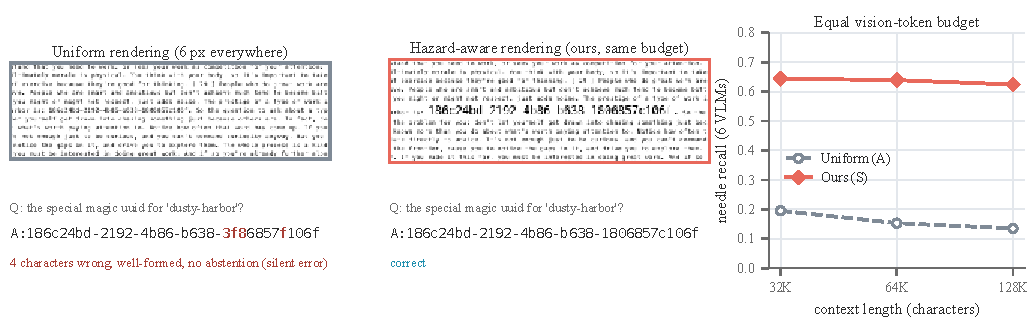
\includegraphics[width=\textwidth]{fig/teaser.pdf}
\captionof{figure}{\textbf{Uniform rendering silently corrupts exactly the strings that must be copied.} A 32K-character essay hides one UUID. \emph{Left:} rendered uniformly at 6\,px, Claude Sonnet 5.5 returns a well-formed UUID with four wrong characters and no sign of doubt. \emph{Middle:} our renderer enlarges the UUID within the same vision-token budget, and the answer is exact. \emph{Right:} needle recall averaged over five VLMs and three RULER tasks. Uniform rendering degrades with context length while hazard-aware rendering does not.}
\label{fig:teaser}
\end{center}
\vspace{0.6em}
}]

\begin{abstract}
Rendering long text into images lets vision-language models (VLMs) read it with several times fewer tokens than the text itself.
This optical compression spends resolution uniformly.
Yet strings that must be copied exactly, such as identifiers and hashes, are misread into well-formed but wrong answers far more often than prose, and they fail more often as contexts grow.
We ask where the pixels should go.
The renderer, unlike the model, sees the text, so it can flag high-entropy strings and draw them larger while drawing prose smaller, within the vision-token budget of uniform rendering.
This allocation is training-free, query-independent, and needs only black-box access to the VLM.
Across five commercial and open-weight VLMs accessed through APIs, it raises RULER needle recall over uniform rendering by 0.55 and 0.43 at the two densest budgets (95\% CIs [0.48, 0.62] and [0.27, 0.56]).
At 32K--128K characters it raises recall by 0.48 while using up to 27\% fewer billed tokens.
Enlarging random words, or boxing the needles without enlarging them, does not help, so the gain comes from legibility of the targeted strings.
The gain shrinks as the budget relaxes and is no larger than a font search at 10\,px.
On LongBench, allocation doubles the recall of naturally occurring identifiers that the detector flags (0.23 to 0.48) without changing QA accuracy relative to uniform rendering; strings the detector misses gain nothing.
For flagged targets, verbatim anchors from prior work are as accurate on the allocated image as on a uniform one, and cheaper wherever allocation shrinks the image.
All image arms remain well below plain text on QA: allocation makes optical compression safer for identifiers, not a substitute for text.
\end{abstract}

\section{Introduction}
\label{sec:intro}

Long contexts are expensive to feed to large models.
Recent work cuts this cost by \emph{rendering} text into images and letting a vision-language model (VLM) read the pixels~\cite{wei2025deepseekocr,cheng2025glyph,rust2023pixel}.
A page of small glyphs costs a fixed number of vision tokens regardless of how many characters it holds, so dense rendering can compress a document several-fold.
In our measurements, a 128K-character essay costs 27.1K billed tokens as text but only 4.7K as a uniformly rendered image (mean of the four readers that report billed usage for both).
The compression needs no training, works with any VLM that accepts images, and is controlled entirely by the party that renders the text.

Existing systems decide \emph{how densely} to render, but rarely \emph{where} the resolution goes.
Optical compressors choose one font, size, and layout for the whole document, sometimes searched for a good accuracy--compression trade-off~\cite{cheng2025glyph}.
Methods that do vary resolution within the input are trained~\cite{zhong2026focusvtc,xu2026seer,xie2026lensvlm} or read the model's attention for each query~\cite{zeng2026agar}.
Visual-token reduction prunes or merges tokens after encoding~\cite{chen2024fastv,yang2025visionzip}.
None of these is available to a party that only renders the text and calls a black-box API.

Uniform resolution hurts some strings far more than others.
\Cref{fig:teaser} shows the typical outcome: a VLM returns a well-formed UUID with four wrong characters and no hedge.
Prior work on failure-aware optical compression~\cite{anon2026renderretain} showed that such silent corruption concentrates in high-entropy spans.
It responded at the level of whole blocks: it flags these spans from the text, copies them verbatim next to the image as \emph{anchors}, and routes risky blocks back to text.
These remedies leave the image itself unchanged.
Same problem found at long-context scale.
At an equal budget, uniform rendering recovers only 8--22\% of RULER needles (mean of five readers, \cref{tab:baselines}), and its recall falls from 0.12 at 32K characters to 0.07 at 128K.

Why do exactly these strings fail?
A VLM that reads rendered text combines two sources of evidence for each character: what the glyph shows, and what its language model expects from the context.
Prose is predictable, so when glyphs blur, the expectation fills the gap.
An identifier is not: its format is predictable, but each hexadecimal character carries 4 bits that only the pixels can supply.
Our readers show this split.
Under uniform rendering they write the four hyphens of a UUID correctly 99\% of the time but its hexadecimal characters only 51\% of the time. For four of five readers, most wrong answers of the right length are not misreadings: they have the right format with nearly every character invented (\cref{sec:why}).
Uniform rendering therefore spends equal pixels on characters the language prior can reconstruct and on characters that only pixels can supply.
When the latter fall below legibility, the reader often fills them in from the prior rather than abstaining, so many errors are silent.

The renderer already holds the signal needed to fix the image.
Before any pixel is drawn, the text shows which strings the prior cannot reconstruct, and the renderer decides how many pixels each string gets.
We propose \emph{\ours} (\cref{fig:method}): flagged high-entropy strings are drawn larger and prose smaller, subject to the image costing no more vision tokens than uniform rendering.
The allocation (arm S in our experiments) is training-free and query-independent, so the same rendering can serve every question about a document.
It composes with the anchors and text routing of prior work~\cite{anon2026renderretain}, which we treat as baselines and building blocks (arms K and X).

Our contributions are:
\begin{itemize}
  \item \textbf{A principle and a rule.} We trace verbatim failures to characters whose content the language prior cannot supply, and propose budget-constrained glyph allocation, which moves pixels to them using only the text and black-box access (\cref{sec:method}). In a controlled study at equal glyph size, each of the three readers we can compare copies a found random hexadecimal string exactly far less often than a found English phrase (e.g., 0.08 vs.\ 0.57 for GPT; \cref{sec:why}).
  \item \textbf{Controlled evidence.} Across five readers, allocation raises needle recall over uniform rendering by 0.43--0.55 at 16K characters and by 0.48 at 32K--128K, and beats font/size search, render-then-downsample, random-word enlargement, and boxing the needles (\cref{tab:pooled}). It turns fabricated answers into read ones. The gain shrinks at milder budgets, and at 10\,px allocation matches font search.
  \item \textbf{Natural strings and side effects.} Allocation doubles the recall of flagged identifiers in LongBench documents (0.23 to 0.48), neither helps nor hurts unflagged digit strings, and leaves LongBench QA unchanged relative to uniform rendering; every image arm still trails plain text.
  \item \textbf{Composition with anchors.} Anchors from prior work are as accurate on the allocated image as on a uniform one and cheaper where allocation shrinks it. On standard needle tasks the anchors contain the answer, so recall there measures copying. Anchors can mislead when the target is not flagged.
\end{itemize}

\section{Related Work}
\label{sec:related}

\paragraph{Optical context compression.}
Reading text from pixels has a long history, from pixel-based language models~\cite{rust2023pixel,gao2024screenshots} to unified image--text encoders~\cite{tschannen2023clippo} and screenshot pretraining~\cite{lee2023pix2struct}.
Recent systems render long contexts to compress them: DeepSeek-OCR decodes text from few vision tokens~\cite{wei2025deepseekocr,wei2026deepseekocr2}, Glyph searches for a good global rendering configuration~\cite{cheng2025glyph}, and other work renders whole inputs, distant context, or interleaved text~\cite{li2025textpixels,xing2025vist,wang2024visincontext}.
Evaluations show where this fails: compressed reading loses retrieval ability~\cite{zhao2025vtcbench}, the text--pixel gap depends on font and resolution~\cite{sun2026reading}, optical compression can underperform mean pooling~\cite{lee2026autoencoding}, and accuracy collapses when linguistic priors are removed~\cite{liang2026visualmerit,gao2026zerosense}.
This last finding is the starting point of our account: what the prior cannot supply must come from the pixels.
Several methods vary resolution within the input, but they are trained (FocusVTC~\cite{zhong2026focusvtc}, SEER~\cite{xu2026seer}, LensVLM~\cite{xie2026lensvlm}; in document understanding, DocOwl2 and TextMonkey~\cite{hu2024docowl2,liu2024textmonkey}).
Among rendering changes, AGAR is the most similar: it re-renders a page and enlarges the word spans that receive the most middle-to-late-layer attention~\cite{zeng2026agar}. It is training-free but needs the model's attention and a first pass for each query.
Our allocation is decided from the text before any model call, works with black-box APIs, and does not depend on the question.
Failure-aware optical compression~\cite{anon2026renderretain} is the closest prior work. It detects high-entropy spans from the text, keeps them as exact text anchors, routes risky blocks to text, and retries on mismatch, but leaves the image unchanged.
We change the image and reuse its anchors and routing as baselines.

\paragraph{Visual-token reduction and text-side compression.}
Training-free pruning and merging reduce the tokens of an encoded image~\cite{chen2024fastv,zhang2025sparsevlm,yang2025visionzip,shang2025prumerge,bolya2023tome,fang2026prunesid,lv2026vprune,zhang2026trio}, including for text-rich and OCR inputs~\cite{wan2026rtprune,li2025fcotvl}.
They act on visual features inside the model, where it is no longer explicit that a group of glyphs forms a hash. We do not test whether pruning keeps the enlarged glyphs.
Prompt compressors drop tokens judged uninformative~\cite{jiang2023llmlingua,jiang2024longllmlingua,li2023selective,pan2024llmlingua2}, learned compressors map context to soft tokens~\cite{mu2023gist,ge2024icae,chevalier2023autocompressors}, and KV-cache methods evict entries~\cite{zhang2023h2o,li2024snapkv,xiao2024streamingllm,devoto2025expected}.
Selective Context, like our detector, uses an information signal, but to \emph{remove} low-information text. We keep every character and only change how large it is drawn.
Caching prompt segments~\cite{gim2024promptcache} is a competing way to cut cost for repeated queries that we do not evaluate.

\paragraph{Evaluation and input resolution.}
We measure verbatim fidelity with RULER~\cite{hsieh2024ruler} and collateral damage with LongBench~\cite{bai2024longbench}. Text-rich benchmarks~\cite{liu2024ocrbench,ma2024mmlongbenchdoc} show the same weakness on natural images and PDFs.
Modern VLMs allocate vision tokens roughly in proportion to pixel area~\cite{wang2024qwen2vl,bai2025qwen25vl,bai2025qwen3vl,chen2024internvl15,li2025llavaonevision}, so the rendering budget is a controllable cost. We report provider-billed tokens.

\section{Method}
\label{sec:method}

% Method overview (TikZ). Palette: peach #F7D8B8, light aqua #BFE6EA, salmon #F6A69A, mist #D9E2EB, warm white #F2F2F2,
% deep teal #1F8FAE, coral #E8685B, dark coral #A83E35.
\begin{figure*}[t]
\centering
\resizebox{\textwidth}{!}{%
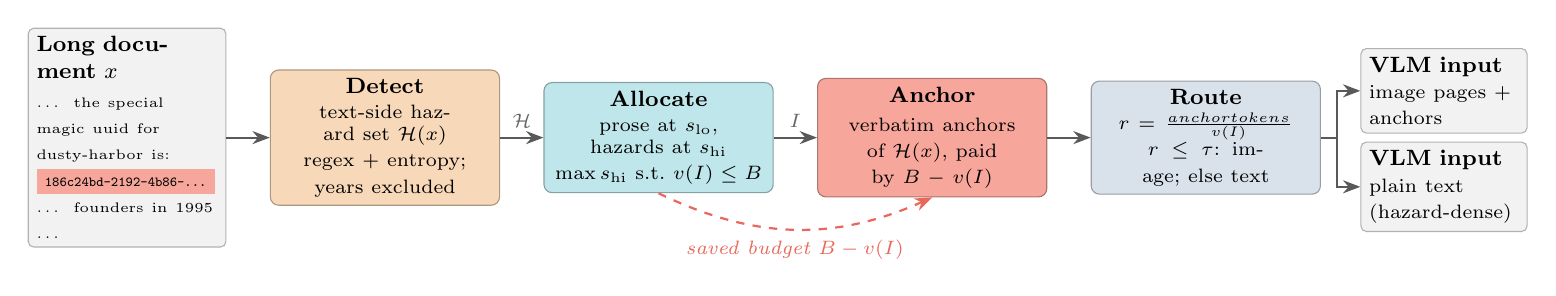
\begin{tikzpicture}[
  font=\footnotesize,
  >={Stealth[length=2.2mm]},
  mod/.style={draw=#1!70!black, fill=#1, rounded corners=3pt, minimum height=1.35cm, text width=2.7cm, align=center, inner sep=3pt},
  io/.style={draw=gray!60, fill=cWarm, rounded corners=2pt, align=left, inner sep=3pt, text width=2.3cm},
  lab/.style={font=\scriptsize\itshape, text=gray!80!black},
  flow/.style={->, thick, draw=gray!70!black},
  save/.style={->, thick, dashed, draw=cCoral},
]
% input
\node[io] (doc) at (0,0) {\textbf{Long document $x$}\\[1pt]
  \tiny \ldots{} the special magic uuid for dusty-harbor is: \colorbox{cSalmon}{\texttt{186c24bd-2192-4b86-\ldots}} \ldots{} founders in 1995 \ldots{}};
% modules
\node[mod=cPeach, right=0.55cm of doc] (det) {\textbf{\textsc{Detect}}\\[1pt]\scriptsize text-side hazard set $\mathcal{H}(x)$\\ regex + entropy; years excluded};
\node[mod=cAqua, right=0.55cm of det] (alloc) {\textbf{\textsc{Allocate}}\\[1pt]\scriptsize prose at $s_{\mathrm{lo}}$, hazards at $s_{\mathrm{hi}}$\\ $\max s_{\mathrm{hi}}$ s.t.\ $v(I)\le B$};
\node[mod=cSalmon, right=0.55cm of alloc] (anc) {\textbf{\textsc{Anchor}}\\[1pt]\scriptsize verbatim anchors of $\mathcal{H}(x)$, paid by $B - v(I)$};
\node[mod=cMist, right=0.55cm of anc] (route) {\textbf{\textsc{Route}}\\[1pt]\scriptsize $r=\frac{\text{anchor tokens}}{v(I)}$\\ $r\le\tau$: image; else text};
% outputs
\node[io, text width=1.9cm, above right=0.05cm and 0.5cm of route.east, anchor=south west] (img) {\textbf{VLM input}\\ \scriptsize image pages + anchors};
\node[io, text width=1.9cm, below right=0.05cm and 0.5cm of route.east, anchor=north west] (txt) {\textbf{VLM input}\\ \scriptsize plain text (hazard-dense)};
% flows
\draw[flow] (doc) -- (det);
\draw[flow] (det) -- node[lab, above] {$\mathcal{H}$} (alloc);
\draw[flow] (alloc) -- node[lab, above] {$I$} (anc);
\draw[flow] (anc) -- (route);
\draw[flow] (route.east) -- ++(0.2,0) |- (img.west);
\draw[flow] (route.east) -- ++(0.2,0) |- (txt.west);
\draw[save] (alloc.south) to[bend right=25] node[lab, below, text=cCoral] {saved budget $B-v(I)$} (anc.south);
\end{tikzpicture}}
\caption{\textbf{Hazard-aware rendering.} \textsc{Detect} marks verbatim-risky strings in the text before rendering; \textsc{Allocate} enlarges only those strings and shrinks prose so that the image never exceeds the vision-token budget $B$ of uniform rendering (a 6\,px uniform image in our experiments); \textsc{Anchor} spends the budget the allocation saved on anchors, verbatim text copies of the flagged strings; \textsc{Route} sends documents whose anchors would be too expensive to plain text. Every step is training-free and needs no access to the model.}
\label{fig:method}
\end{figure*}


\paragraph{Overview.}
Given a long document, an optical compressor renders it into image pages that a VLM reads in place of the text.
Our goal is to make the strings that must be copied exactly survive this rendering, without spending more vision tokens and without access to the model.
\Cref{fig:method} shows the pipeline.
\textsc{Detect} reads the text and marks verbatim-hazardous strings.
\textsc{Allocate}, our contribution, renders those strings large and the remaining prose small, so that the image costs no more than uniform rendering.
The other two steps follow prior work on failure-aware optical compression~\cite{anon2026renderretain}.
\textsc{Anchor} appends verbatim text copies of the flagged strings, paid for here by the vision tokens that allocation saves.
\textsc{Route} falls back to plain text when the anchors would be too expensive.

\subsection{Problem formulation}
\label{sec:formulation}

A document $x=(w_1,\dots,w_n)$ is a sequence of whitespace-separated words.
A renderer $R$ maps $x$ and a size assignment $\sigma:\{1,\dots,n\}\to\mathbb{N}$ (glyph height in pixels for every word) to an image $I=R(x;\sigma)$ of fixed width, which is split into pages for the VLM.
To compare renderings, we need their cost in the unit providers bill.
Following the patch-based accounting of dynamic-resolution VLMs~\cite{wang2024qwen2vl}, we define the vision-token cost of an image with pages of width $w_p$ and height $h_p$ as
\begin{equation}
  v(I) \;=\; \sum_{p} \left\lceil \tfrac{w_p}{28} \right\rceil \left\lceil \tfrac{h_p}{28} \right\rceil ,
  \label{eq:vtok}
\end{equation}
where each vision token covers a $28\times28$-pixel area (14-pixel patches merged $2\times2$ in Qwen2-VL).
\Cref{eq:vtok} is used only to enforce budgets; all costs we report are the prompt tokens billed by each provider.
The \emph{budget} is the cost of uniform rendering at a base size $s_0$, $B = v\big(R(x;\sigma\equiv s_0)\big)$.
Every method we compare uses the same number of vision tokens as the uniform baseline, up to page rounding.
Let $\mathcal{H}(x)\subseteq\{1,\dots,n\}$ be the indices of hazardous words, those whose value is needed verbatim downstream.
We seek a size assignment that makes every $w_i$, $i\in\mathcal{H}(x)$, as legible as possible subject to $v(I)\le B$, without deleting or reordering any character.

\subsection{Where pixels matter}
\label{sec:principle}

Which words should receive the pixels?
Consider how a reader copies a string $c_1\dots c_L$ from the image.
As a schematic model, the reader combines two terms for each character: visual evidence from the glyph, which grows with the glyph size $s$, and the expectation of its language model given the context:
\begin{equation}
  p(c_i \mid I, \mathrm{ctx}) \;\propto\; \underbrace{p(I_i \mid c_i;\, s_i)}_{\text{pixels}} \; \underbrace{p_\theta(c_i \mid \mathrm{ctx})}_{\text{language prior}} .
  \label{eq:reading}
\end{equation}
The pixels must supply whatever the prior leaves open, roughly the \emph{residual entropy} $H(c_i \mid \mathrm{ctx})$ of each character.
For English prose this is small, because most letters are predictable from the words around them.
For the hyphens of a UUID it is close to zero.
For its hexadecimal characters it is 4 bits, all of which must come from the glyph.
Exact copying fails if any single character fails, so a string is only as legible as its least predictable character.
Uniform rendering gives every character the same visual evidence, which is more than prose needs and, at dense budgets, less than an identifier needs.
When the evidence for a high-entropy character is too weak, the prior dominates \cref{eq:reading}. The prior knows the format but not the content, so we expect the reader to emit a well-formed string with invented characters.
Under a fixed budget, pixels should therefore move from characters with low residual entropy to characters with high residual entropy.
The trade is favorable because the two kinds of characters sit on different parts of their legibility curves.
Predictable text is on the flat part: in our controlled study, found English phrases keep 92--96\% character accuracy from 10 down to 4\,px, so taking pixels from prose costs little.
High-entropy strings at dense budgets are on the steep part: giving a UUID 12 instead of 5--6\,px raises its hexadecimal accuracy from 51\% to 91\% (\cref{sec:why}).
A small loss where the prior compensates buys a large gain where it cannot.
Under the patch convention of \cref{eq:vtok}, a 6\,px Menlo character is 4 pixels wide. One 14-pixel patch then mixes about 3.5 characters, and one vision token covers 7 characters on each of 3 lines; at 12\,px a patch holds 2 characters.
The two steps below implement this principle with simple means: a text-side proxy for residual entropy (\textsc{Detect}) and a two-level size assignment (\textsc{Allocate}).

\subsection{\textsc{Detect}: text-side hazard detection}
\label{sec:detect}

The detector approximates $\mathcal{H}(x)$ without labels, following the regex-plus-windowed-entropy design of~\cite{anon2026renderretain}.
Its premise is that a string is hazardous when it is \emph{high-entropy}: a misread character yields another valid-looking string, and the language model cannot repair it from context.
After stripping surrounding punctuation, we flag a word if it matches one of five patterns: a hexadecimal run of at least 8 characters, a run of at least 5 digits, a path containing a digit or a file extension, an IP address, or a digest prefix.
We also flag words that mix letters and digits and either have at least 20 identifier characters or contain a 16-character window with Shannon entropy of at least 3.5 bits.
Two choices encode what \emph{not} to protect.
Four-digit numbers are excluded because in natural text they are mostly years, which are low-entropy and cheap to read.
The length and entropy rules require mixed letter--digit tokens so that long English words are not flagged.
These exclusions are our changes.
A preliminary detector without them flagged 85--112 words per LongBench document on average, most of them years, and shrank prose in documents that did not need it (\cref{app:negative}).

When the detector flags nothing, the rendering is identical to the uniform baseline, so a document whose hazards all go undetected loses only the potential gain (\cref{sec:niq}).
A missed hazard in a document where \emph{other} strings are flagged, however, shrinks together with the prose.

\subsection{\textsc{Allocate}: budget-constrained glyph allocation}
\label{sec:allocate}

Given $\mathcal{H}(x)$, we restrict size assignments to two levels: prose words at $s_{\mathrm{lo}}$ and flagged words at $s_{\mathrm{hi}}$.
Prose is wrapped at character boundaries, as in the uniform baseline; each flagged word is kept whole on one line.
We choose the sizes by
\begin{equation}
\begin{aligned}
  (s_{\mathrm{hi}}^{\ast}, s_{\mathrm{lo}}^{\ast}) = &\operatorname*{lexmax}_{\substack{s_{\mathrm{hi}}\in[s_0,\,12]\\ s_{\mathrm{lo}}\in[5,\,\min(s_{\mathrm{hi}},s_0)]}} (s_{\mathrm{hi}}, s_{\mathrm{lo}})\\
  &\text{s.t.}\;\; v\big(R(x;\sigma_{s_{\mathrm{lo}},s_{\mathrm{hi}}})\big)\le B ,
\end{aligned}
  \label{eq:alloc}
\end{equation}
where $\sigma_{s_{\mathrm{lo}},s_{\mathrm{hi}}}$ assigns $s_{\mathrm{hi}}$ to words in $\mathcal{H}(x)$ and $s_{\mathrm{lo}}$ to all others, and $\operatorname{lexmax}$ first maximizes $s_{\mathrm{hi}}$ and then $s_{\mathrm{lo}}$.
The order follows \cref{sec:principle}: the marginal pixel is worth more on a hash than on prose.
The lower bound of 5\,px keeps prose within the range VLMs still read, and $s_{\mathrm{lo}}\le s_0$ ensures prose is never enlarged.
If no pair with $s_{\mathrm{hi}}>s_{\mathrm{lo}}$ fits, prose-only lines lose one pixel of line spacing and the search is repeated; at $s_0=5$\,px this is what makes room (\cref{app:alloc}).
If $\mathcal{H}(x)=\emptyset$, the result is identical to uniform rendering.
Allocation takes about 1\,s for 32K and 4\,s for 128K characters on one CPU core.

\subsection{\textsc{Anchor} and \textsc{Route}}
\label{sec:anchor}
\label{sec:route}

When prose can shrink ($s_0=6$\,px), the allocated image usually ends \emph{below} the budget, because the search stops at the largest feasible $s_{\mathrm{hi}}$ rather than filling every remaining row.
In our long-context runs, it used 13--27\% fewer billed tokens than uniform rendering.
Following~\cite{anon2026renderretain}, we spend these savings on \emph{anchors}: after the question, the flagged strings are appended verbatim as text, under a line stating that they are copied exactly from the image.
Anchors carry no key, but a document with only one or a few flagged strings yields a short list that may consist of the answer alone.
A reader can then answer without reading the image (\cref{sec:anchors}).
Anchor cost grows linearly with the number of flagged strings, so before any model call we compute the ratio
\begin{equation}
  r(x) \;=\; \frac{\sum_{i\in\mathcal{H}(x)} c(w_i)}{v(I)}, \qquad c(w) = \tfrac{|w|}{2} + 3,
  \label{eq:route}
\end{equation}
where $c(w)$ estimates the text tokens of one anchor and $I$ is the allocated image, and send the document as plain text when $r(x)>\tau$.
This replaces the density test of~\cite{anon2026renderretain} with one that accounts for the allocated image.
We use $\tau=0.3$, the median of per-reader two-fold cross-validation on a synthetic density sweep (\cref{app:density}).

\section{Experimental Setup}
\label{sec:setup}

\paragraph{Readers.}
We treat every VLM as a black box and query it with one stateless request per item at temperature 0 (0.01 for MiniMax); a request whose output cannot be parsed is re-sent up to three times.
The six readers span vendors, scales, and open weights: Claude Sonnet 5.5, Gemini 3.5 Flash-Lite, GPT-6 Luna (minimal reasoning effort), Qwen3-VL-235B-A22B~\cite{bai2025qwen3vl}, Llama 4 Maverick, and MiniMax-M3.
Costs are the prompt tokens billed by each provider, which include the image, the question, and any appended copy; MiniMax does not report usage and is excluded from cost averages only.
Empty responses and transport errors (73 of about 33{,}000 calls in all experiments reported here) are dropped; any other unparseable output, including refusals and degenerate repetition, counts as wrong.

\paragraph{Tasks.}
Verbatim fidelity is measured with RULER needle-in-a-haystack tasks~\cite{hsieh2024ruler}, re-implemented with the official templates and Paul Graham essays as the haystack: \emph{single} (one UUID value), \emph{multi-key} (four keys, one queried, numeric values), and \emph{multi-value} (four numeric values for one key).
Contexts have 16K characters (\cref{sec:main}), 32K--128K characters split into up to three pages (\cref{sec:length}), or 32K characters with $k\in\{1,\dots,256\}$ UUID needles to vary hazard density (\cref{sec:density}).
Collateral damage on ordinary comprehension is measured on LongBench~\cite{bai2024longbench} MultiFieldQA-en and HotpotQA (from the length-balanced LongBench-E split), with non-ASCII characters replaced by ``?'', using contexts of at most 40K characters so that one image holds a document; these samples were drawn after the detector was finalized.
We use $N=25$ items per task and reader for RULER at 16K and 32K characters, $N=20$ for the 32K--128K length study, and $N=50$ for LongBench.

\paragraph{Arms.}
All image arms share the renderer of \cref{sec:method}, a 1008-pixel page width, and the budget $B$ of uniform rendering at $s_0\in\{5,6\}$\,px ($\approx$32 and 21 characters per vision token on our long documents).
\textbf{A} is uniform rendering.
\textbf{U} searches font family (monospace, Arial, Arial Narrow) and size for the largest uniform text that fits $B$, a training-free stand-in for global configuration search~\cite{cheng2025glyph}.
\textbf{Z} renders at 10\,px and downsamples the image to $B$, the resolution-compression view of optical encoders~\cite{wei2025deepseekocr}.
\textbf{K} appends anchors, verbatim copies of the flagged strings, to A.
\textbf{S} is our allocation (\cref{sec:allocate}), \textbf{X} adds anchors to S (\cref{sec:anchor}), and \textbf{T} gives the plain text.
Prompts follow the task templates, with the context replaced by the image; RULER answers are requested as JSON.

\paragraph{Metrics and statistics.}
RULER is scored by recall of the gold values (string match, all values), LongBench by token-level F1, as in the original benchmarks.
For every comparison we compute the mean paired difference over items with a 95\% bootstrap confidence interval (10{,}000 resamples) and call a cell significant when the interval excludes zero; a \emph{cell} is one reader on one task at one setting.

\section{Results}
\label{sec:results}

\begin{table*}[t]
\centering
\caption{\textbf{Equal-budget comparison on RULER needle retrieval (16K characters).} Recall averaged over three NIAH tasks ($N{=}25$ each) per reader, at two rendering densities (uniform 5\,px $\approx$ 21 and 6\,px $\approx$ 14 characters per vision token). A, U, Z, and S are images with the same vision-token budget; \textbf{bold} marks the best among them. K adds anchors (verbatim text copies of the flagged strings) to A and is shown in gray because it spends extra text tokens. The last row is the provider-billed prompt-token count averaged over the readers that report usage. Hazard-aware rendering (S) is significantly worse than U or Z in none of the 72 paired comparisons (36 reader$\times$task$\times$density cells $\times$ 2 baselines) and significantly better in 63.}
\label{tab:baselines}
\small
\setlength{\tabcolsep}{4.2pt}
\begin{tabular}{l ccccc ccccc}
\toprule
& \multicolumn{5}{c}{5\,px budget ($\approx$21 chars/vtok)} & \multicolumn{5}{c}{6\,px budget ($\approx$14 chars/vtok)} \\
\cmidrule(lr){2-6}\cmidrule(lr){7-11}
Reader & A & U & Z & S (ours) & \textcolor{gray}{K} & A & U & Z & S (ours) & \textcolor{gray}{K} \\
\midrule
Claude Sonnet 5.5 & 0.14 & 0.22 & 0.19 & \textbf{0.79} & \textcolor{gray}{0.95} & 0.57 & 0.64 & 0.46 & \textbf{0.92} & \textcolor{gray}{1.00} \\
Gemini 3.5 Flash-Lite & 0.41 & 0.57 & 0.79 & \textbf{1.00} & \textcolor{gray}{1.00} & 0.88 & 0.78 & 0.84 & \textbf{1.00} & \textcolor{gray}{1.00} \\
GPT-6 Luna & 0.02 & 0.03 & 0.02 & \textbf{0.50} & \textcolor{gray}{0.91} & 0.11 & 0.16 & 0.08 & \textbf{0.65} & \textcolor{gray}{0.82} \\
Qwen3-VL-235B & 0.00 & 0.00 & 0.00 & \textbf{0.55} & \textcolor{gray}{1.00} & 0.07 & 0.08 & 0.03 & \textbf{0.60} & \textcolor{gray}{1.00} \\
Llama 4 Maverick & 0.00 & 0.00 & 0.00 & \textbf{0.58} & \textcolor{gray}{0.97} & 0.00 & 0.01 & 0.00 & \textbf{0.59} & \textcolor{gray}{0.90} \\
MiniMax-M3 & 0.00 & 0.00 & 0.00 & \textbf{0.57} & \textcolor{gray}{1.00} & 0.02 & 0.01 & 0.00 & \textbf{0.42} & \textcolor{gray}{0.97} \\
\midrule
\textit{Mean} & 0.09 & 0.14 & 0.17 & \textbf{0.66} & \textcolor{gray}{0.97} & 0.28 & 0.28 & 0.23 & \textbf{0.70} & \textcolor{gray}{0.95} \\
\textit{Billed tokens} & 779 & 775 & 768 & 779 & \textcolor{gray}{823} & 913 & 891 & 887 & 812 & \textcolor{gray}{960} \\
\bottomrule
\end{tabular}
\end{table*}


\subsection{Equal-budget comparison}
\label{sec:main}

\Cref{tab:baselines} compares all image arms at the same vision-token budget on 16K-character RULER documents.
Averaged over five readers, uniform rendering recovers 8\% of needles at the denser budget and 22\% at the lighter one.
Claude Sonnet 5.5 (0.57) and Gemini (0.88) are the only readers above 0.11 at 6\,px.
Allocation (S) raises the mean to 0.64 and 0.65, a pooled gain of 0.55 and 0.43 whose confidence intervals exclude zero by a wide margin (\cref{tab:pooled}).
After Holm correction, the gain is significant in 14 and 11 of 15 cells and never significantly negative.
The two stronger uniform baselines barely help: font/size search (U) reaches 0.12 and 0.21, and render-then-downsample (Z) 0.16 and 0.19.
Both plausibly fall short because they spread legibility evenly over all characters.
At 6\,px, S is also 8\% cheaper than uniform rendering (842 vs.\ 920 billed tokens), because prose shrinks more than the enlarged strings grow.
The weaker readers gain most (at 6\,px Llama 4 Maverick from 0.00 to 0.59, GPT from 0.11 to 0.65), while Gemini, already at 0.88, gains 0.12.
Under the precision-aware F1, which penalizes returning several candidate values, the gains are smaller (0.46 and 0.34 pooled) but remain significant in at least 9 of 15 cells.

\paragraph{Targeting, enlargement, or salience?}
Two controls separate the ingredients of S.
Arm R runs the same allocation on randomly chosen ordinary words, matched in total length, so its sizes and cost are close to those of S while the needles shrink with the prose.
R recovers 0.10 of the needles at both budgets, and S exceeds it by 0.54 and 0.56.
Arm B keeps every glyph at the uniform size but draws a box around each flagged string, which makes the needle easy to \emph{find} but not easier to \emph{read}.
B is 0.53 below S and slightly worse than uniform rendering ($-$0.05, CI upper bound $-$0.001; \cref{tab:pooled}), perhaps because the box line touches the small glyphs.
The gain therefore comes from making the targeted strings legible, not from layout changes or from pointing at the needle.

\begin{table}[t]
\centering
\caption{\textbf{Pooled effects} over the five non-Claude readers (recall unless noted). CI: 95\% bootstrap over readers and items. Sig.: cells (reader $\times$ task) significantly positive after Holm correction within each row; neg.: significantly negative.}
\label{tab:pooled}
\footnotesize
\setlength{\tabcolsep}{2.5pt}
\begin{adjustbox}{max width=\columnwidth}
\begin{tabular}{l c c c c}
\toprule
Comparison & $\Delta$ & 95\% CI & sig. & neg. \\
\midrule
\multicolumn{5}{l}{\textit{Equal budget, RULER}} \\
\name $-$ COC, 16K, 5\,px & +0.55 & [+0.48, +0.62] & 14/15 & 0 \\
\name $-$ COC, 16K, 6\,px & +0.43 & [+0.27, +0.56] & 11/15 & 0 \\
\name $-$ COC, 32K--128K, 6\,px & +0.48 & [+0.43, +0.53] & 35/45 & 0 \\
\name $-$ font search, 6\,px & +0.44 & [+0.31, +0.55] & 11/15 & 0 \\
\name $-$ random words, 6\,px & +0.56 & [+0.47, +0.64] & 12/15 & 0 \\
box $-$ COC, 6\,px & -0.05 & [-0.13, 0.00] & 0/15 & 1 \\
\name $-$ box, 6\,px & +0.53 & [+0.41, +0.64] & 14/15 & 0 \\
half $-$ COC, 5\,px & +0.30 & [+0.21, +0.40] & 9/10 & 0 \\
half $-$ COC, 6\,px & +0.21 & [0.00, +0.39] & 8/10 & 0 \\
\name $-$ half, 6\,px & +0.31 & [+0.20, +0.41] & 6/10 & 0 \\
\midrule \multicolumn{5}{l}{\textit{Milder budgets (32K)}} \\
\name $-$ COC, 10\,px & +0.20 & [+0.11, +0.30] & 4/10 & 0 \\
\name $-$ font search, 10\,px & +0.04 & [-0.04, +0.12] & 1/10 & 1 \\
\midrule \multicolumn{5}{l}{\textit{Natural strings (LongBench documents)}} \\
\name $-$ COC, flagged targets & +0.25 & [+0.12, +0.38] & 4/5 & 0 \\
\name $-$ COC, detector-indep. & -0.01 & [-0.11, +0.08] & 0/5 & 0 \\
\midrule \multicolumn{5}{l}{\textit{Ordinary comprehension (LongBench F1)}} \\
\name $-$ COC & +0.02 & [-0.02, +0.06] & 0/10 & 0 \\
\name+anchor $-$ text & -0.21 & [-0.29, -0.13] & 0/10 & 9 \\
\midrule \multicolumn{5}{l}{\textit{Post-processing: {\name}+anchor $-$ COC+anchor (all settings: \cref{tab:app_pooled,tab:app_pooled2})}} \\
RULER 16K, 6\,px (F1) & +0.04 & [0.00, +0.08] & 1/15 & 0 \\
multi-key 64K--128K (F1) & -0.01 & [-0.05, +0.03] & 0/10 & 0 \\
natural, flagged, 6\,px & +0.02 & [-0.06, +0.10] & 0/5 & 0 \\
\bottomrule
\end{tabular}
\end{adjustbox}
\end{table}


\subsection{Why does allocation work?}
\label{sec:why}

\begin{figure}[t]
\centering
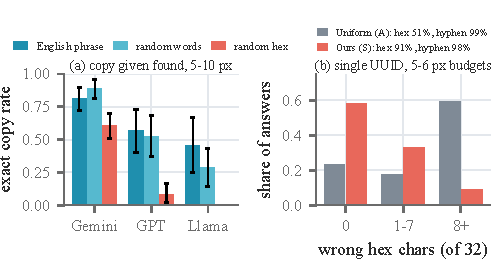
\includegraphics[width=\columnwidth]{fig/why.pdf}
\caption{\textbf{Reading is limited by what the language prior cannot supply.} (a) Controlled study: 32-character targets of three types hidden in the same 16K-character documents and rendered uniformly at 5--10\,px. Among answers in which the reader found the target, the share copied exactly (95\% CI), for the three readers that found enough targets of every type. (b) Single-UUID needles at the 5 and 6\,px budgets: wrong hexadecimal characters per answer of the right length. Under uniform rendering most such answers are fabricated, and under allocation most are exact.}
\label{fig:why}
\end{figure}

\Cref{sec:principle} predicts that readers fail where the pixels must supply what the language prior cannot.
Three observations on the single-UUID needles of \cref{tab:baselines} (five readers, both budgets, and the box runs) are consistent with this.

\emph{The format is read, the content is not.}
Under uniform rendering, a third of the answers are empty.
In the answers of the right length, the four hyphens, which the UUID format predicts, are correct 99\% of the time, but the 32 hexadecimal characters only 51\% of the time.
Allocation raises the hexadecimal characters to 91\% and leaves the hyphens at 98\%. The gain holds for every reader (from 0.15--0.96 to 0.82--1.00).

\emph{Wrong answers are fabricated, not misread.}
If uniform rendering merely blurred a few glyphs, errors would be spread over a few characters.
Instead, 59\% of the right-length answers have at least 8 of 32 characters wrong, with a median of 27, close to the 30 expected from guessing (\cref{fig:why}b). Only 23\% are exact.
The weaker readers drive this pooled pattern. All right-length answers of Llama and MiniMax, and most of those of Qwen and GPT, reproduce the format and invent the content, consistent with \cref{eq:reading}. Gemini, the strongest reader, almost never fabricates and errs by misreading (\cref{app:why}).
Under allocation, 58\% of the answers are exact and 9\% are fabricated.
Among partial misreads under uniform rendering, the most frequent confusion is 8$\to$0 (24 of 89 wrong characters). The two glyphs differ by a small stroke, which a patch holding three or four characters blurs.

\emph{The pixels needed depend on predictability.}
To test this, we hid one 32-character value in the same RULER documents (16K characters) and varied only its type: an English phrase from LongBench passages, random common words, or random hexadecimal characters.
Each document was rendered uniformly at 4--10\,px. We scored the answers in which the reader found the target (at least 50\% similar to it), which separates transcription from search (\cref{app:why}).
MiniMax and Qwen3-VL rarely found English or word targets and usually answered with the key instead, so we compare transcription for the three readers that found enough targets of every type.
For each of them, a found hexadecimal string is copied exactly far less often than a found English phrase at 5--10\,px: 0.61 vs.\ 0.82 for Gemini, 0.08 vs.\ 0.57 for GPT, and 0.00 vs.\ 0.46 for Llama (\cref{fig:why}a). Random words reach 0.89, 0.53, and 0.29.
Hexadecimal and English targets also differ in their glyphs, so this test supports but does not isolate the role of the prior (\cref{app:why}).

The account is also consistent with the boundaries of \cref{tab:pooled}: boxing does not help, suggesting legibility rather than search alone is the bottleneck; at 10\,px font/size search recovers most of the gain (S$-$U $+$0.04); dense hazards leave too few pixels to lift any string (\cref{app:density}); and shrinking prose costs little (\cref{sec:longbench}).

\subsection{Scaling with context length}
\label{sec:length}

\begin{figure}[t]
\centering
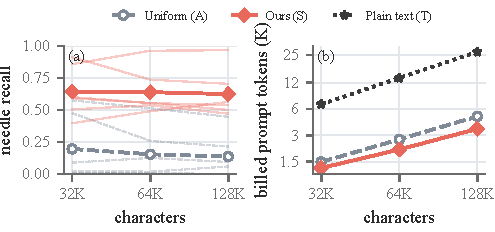
\includegraphics[width=\columnwidth]{fig/scaling.pdf}
\caption{\textbf{Context length.} RULER at 32K--128K characters (6\,px budget, up to three image pages, $N{=}20$ per task). (a) Needle recall; thin lines are individual readers (including Claude), thick lines the mean over five readers. (b) Billed prompt tokens averaged over the four of these readers that report usage; log scale.}
\label{fig:scaling}
\end{figure}

Optical compression is most attractive for long documents, so \cref{fig:scaling} extends the comparison to 128K characters.
Under uniform rendering, mean recall declines from 0.12 at 32K to 0.08 at 64K and 0.07 at 128K, consistent with reports that compressed reading loses retrieval ability as context grows~\cite{zhao2025vtcbench}.
Allocation stays between 0.60 and 0.56, a pooled gain of 0.48 [0.43, 0.53] with 35 of 45 cells significant after Holm correction.
It also uses 13\%, 23\%, and 27\% fewer billed tokens than uniform rendering at the three lengths.
On the four readers with billed costs for both, it uses 5.4$\times$, 6.8$\times$, and 8.0$\times$ fewer than plain text, which every reader answers with recall of at least 0.99.
Individual readers differ widely (0.47 to 0.97 at 128K for S; \cref{tab:app_length}).

\subsection{Milder budgets}
\label{sec:regime}

Our main budgets put most readers near the floor of uniform rendering, where gains are easiest to obtain.
We therefore repeated the single and multi-key tasks at 32K characters with base sizes of 8 and 10\,px, which cost 1.5 and 2.3 times as many vision tokens as 6\,px.
Uniform rendering improves with size (multi-key: 0.26 at 8\,px, 0.60 at 10\,px), and the gain of S shrinks accordingly, to 0.38 at 8\,px and 0.20 at 10\,px (\cref{tab:pooled}).
The font/size search catches up: S beats U by 0.26 at 8\,px but only by 0.04 at 10\,px, which is not significant.
Single UUIDs remain hard even here (A 0.20, S 0.44 at 10\,px).
Allocation is most useful where the budget is tight, which is also where optical compression saves the most.

\subsection{Naturally occurring strings}
\label{sec:niq}


RULER needles are synthetic, and our detector was designed with such strings in mind.
We built two sets of 60 questions from LongBench documents of up to 40K characters (ten each from six tasks).
Each asks for the exact string that follows a unique six-word phrase (\cref{app:niq}).
In the first set, targets are strings the detector flags, such as report and grant numbers, ISBNs, citation keys, and URLs.
Here allocation doubles mean recall (0.23 to 0.48, significant for four of five readers) at 12\% fewer billed tokens than uniform rendering (\cref{tab:niq}).
In the second set, targets are any digit-bearing tokens of at least four characters, sampled without the detector.
The detector flags only one of the 60, because most are short numbers, percentages, and version strings such as ``25,000'' or ``2.0.13''.
On these, every image arm is poor (0.36--0.45 against 0.96 for text), and allocation neither helps nor hurts ($-$0.01 [$-$0.11, 0.08]).
Shrinking prose to make room for flagged strings thus did not measurably damage the strings the detector misses, but nothing in the image protects them either.
A synthetic detector ablation agrees: needles the regex misses leave S at uniform recall (0.33 vs.\ 0.32), while an oracle detector would reach 0.82 (\cref{tab:detector}).

\subsection{Anchors on the allocated image}
\label{sec:anchors}

Anchors~\cite{anon2026renderretain} copy the flagged strings into the prompt.
In the essay haystacks of \cref{tab:baselines}, the only flagged strings are the needles. The anchor list \emph{is} then the answer, and K and X reach 0.90--1.00 by copying. On multi-key, readers often return the whole list (F1 0.46--0.52; \cref{app:rescore}).
We therefore compare K and X on the flagged natural identifiers, where documents carry 5.3 distinct anchors and a random pick would score 0.44.
Across base sizes of 5, 6, and 7\,px, X reaches 0.75--0.81 and lies on or above K's recall--cost frontier by 0.02--0.05, though no pooled interval excludes zero (\cref{app:anchors}).
At 64K--128K characters, X costs 29--31\% less than K, but under F1 the anchors add nothing over allocation alone.
When the target is not flagged, anchors can mislead (X 0.36 vs.\ 0.44 for S and K on the detector-independent set).
Beyond about 16 flagged strings per 32K characters, anchors on either image become expensive and ineffective, and routing to text~\cite{anon2026renderretain} takes over. On real corpora, prose goes to images and code and logs to text (\cref{app:density,app:corpora}).

\subsection{Effect on ordinary comprehension}
\label{sec:longbench}


Shrinking prose could hurt questions unrelated to identifiers.
On held-out LongBench documents of up to 40K characters (\cref{tab:longbench}), pooled F1 changes by +0.02 [$-$0.02, 0.06] for S and +0.02 [$-$0.03, 0.07] for X relative to uniform rendering, which rules out losses larger than about 0.03 (\cref{tab:pooled,tab:app_pooled2}). One reader--task cell is significantly negative for S, and none for X.
Relative to plain text, however, every image arm loses: X trails it by 0.15--0.33 F1 in 9 of 10 cells, at a fifth to a quarter of the text cost.
Allocation thus removes a failure specific to identifiers but does not make optical compression a substitute for text.


\section{Limitations and Conclusion}
\label{sec:conclusion}

\paragraph{Limitations.}
Our fidelity evaluation relies mainly on synthetic needles inserted into natural text; LongBench establishes that the method does no harm on natural documents but not how much it helps on their identifiers, for lack of a benchmark that asks for verbatim copies of naturally occurring strings.
We evaluate black-box readers only and therefore cannot say how enlarged glyphs change a model's internal attention.
Budgets follow one patch-based accounting rule (\cref{eq:vtok}); providers tile images differently, and while billed costs confirm the savings for the readers we tested, other tokenizers may shift them.
The detector is rule-based: it is fail-safe but recall-bounded, and hazards it does not recognize receive no protection.
Finally, reallocation alone raises recall without reducing the share of confident near-misses; only anchors remove them.

\paragraph{Conclusion.}
Optical context compression decides how many pixels a document receives but not where they go, and its failures concentrate on exactly the strings that must survive verbatim.
Because the renderer reads the text before it draws it, it can spend resolution where errors hurt, reinvest the savings in anchors, and fall back to text when a document is too dense with identifiers.
These steps are training-free and model-agnostic, and across six VLMs they make optical compression reliable for embedded identifiers: on long documents with few identifiers, the routed system retrieves them nearly as well as plain text at about one fifth of its cost, and it sends identifier-dense documents to text.


{
    \small
    \bibliographystyle{ieeenat_fullname}
    \bibliography{refs}
}

\section*{LLM Usage Statement}
Large language models play two roles in this work.
First, they are the \emph{objects of study}: the six vision-language models listed in \cref{sec:setup} and the additional Claude reader of \cref{app:claude} were queried as black-box readers, and all reported numbers are computed by our scripts from their logged outputs.
Second, the authors used an LLM-based coding assistant (Claude) to help implement the rendering and evaluation code, to generate figures and tables from the logged results, and to draft and edit the text of this paper.
The assistant also proposed experiments and analyses, which the authors reviewed and approved; the authors take responsibility for all claims. Every number in the paper is produced programmatically from the experiment logs, and every reference was checked against its primary source.
No LLM was used to generate or label evaluation data beyond the readers' answers being evaluated.


% Supplementary material: compiled together for cross-references, then split by build_pdfs.sh
\clearpage
\onecolumn
\setcounter{page}{1}
\begin{center}
{\Large\textbf{Spend Pixels Where It Hurts:}}\\[0.2em]
{\Large\textbf{Hazard-Aware Rendering for Optical Long-Context Compression}}\\[0.5em]
{\Large Supplementary Material}
\end{center}
\vspace{0.5em}
% citations in the supplementary do not add page back-references to the main reference list
\makeatletter\renewcommand*{\Hy@backout}[1]{}\makeatother
\appendix
\section{Implementation Details}
\label{app:impl}

\paragraph{Renderer.}
Pages are 1008 pixels wide (36 patches) with a 4-pixel margin and are rendered in grayscale with the Menlo monospace font through PIL.
Prose is wrapped at character boundaries; a flagged word is placed whole on the next line when it does not fit.
Each line is as tall as its largest glyph plus one pixel of leading.
Documents taller than 2016 pixels are split into pages at blank pixel rows, so no line is cut; all pages are sent in one request in reading order.
The budget of \cref{eq:vtok} is enforced on the unsplit image; splitting can add one patch row per page, which made 10 of the 180 reallocated long-context images 1.2\% more expensive than their uniform counterparts.
All reported costs are billed tokens and include this effect.

\paragraph{Detector.}
After stripping the characters \texttt{.,;:()[]"'} from both ends, a word is flagged if it matches \verb![0-9a-f]{8,}!, \verb!\d{5,}!, \verb!/\S*\d\S*!, \verb!\d+\.\d+\.\d+\.\d+!, \verb!\S+/\S+\.\w{1,5}!, or \verb!sha256=!, or if it contains at least one letter and one digit and either contains \verb![A-Za-z0-9_\-]{20,}! or is at least 16 characters long with a 16-character window whose character entropy is at least 3.5 bits.

\paragraph{Baselines.}
U tries Menlo, Arial, and Arial Narrow at sizes 14 down to 5\,px and keeps the largest size that fits the budget (ties broken by font order); at the 5\,px and 6\,px budgets it selects 6\,px Arial and 8\,px Arial Narrow for most documents.
Z renders at 10\,px and shrinks the image by repeated factors of 0.98 with Lanczos resampling until it fits the budget (final scale 0.52--0.64).
For RULER and the natural-identifier questions, K and X append, after the question, the line ``Exact strings copied verbatim from the text block in the image:'' followed by one flagged string per line; for LongBench, the anchors are inserted after the image placeholder and before the question, under ``Exact strings copied verbatim from the text in the image:''.

\paragraph{Prompts and scoring.}
RULER prompts follow the official template with the context replaced by ``[The text is rendered in the image above.]'', add ``Copy each one exactly, character for character.'', and ask for a JSON list of values; a gold value counts as recalled if it appears (case-insensitively) in any returned string.
LongBench prompts are the official ones for each task; the first output line is scored with the official QA F1.
For the plain-text arm the context is inserted verbatim into the same template.

\paragraph{Router threshold.}
$\tau$ is chosen per reader by two-fold cross-validation on the density sweep (folds by item parity), maximizing recall minus 0.5 times the cost relative to plain text over $\tau\in\{0,0.05,0.1,0.2,0.3,0.5,0.75,1,1.5,2,4,\infty\}$.
Selected values were 0.1--0.5 with median 0.3, which we use for all other experiments. The frontier in \cref{fig:density}c sweeps $\tau$ and the per-density figures use the median $\tau$; both are therefore in-sample, unlike the cross-validated aggregate.

\section{Per-Reader Results}
\label{app:tables}

\Cref{tab:app_length,tab:app_density} give per-reader numbers for \cref{fig:scaling,fig:density}.

\begin{table}[!htbp]
\centering\small\setlength{\tabcolsep}{4pt}
\caption{Per-reader recall for the length study (\cref{fig:scaling}). The mean excludes Claude.}
\label{tab:app_length}
\begin{tabular}{l cc cc cc}
\toprule
& \multicolumn{2}{c}{32K} & \multicolumn{2}{c}{64K} & \multicolumn{2}{c}{128K} \\
\cmidrule(lr){2-3}\cmidrule(lr){4-5}\cmidrule(lr){6-7}
Reader & A & S & A & S & A & S \\
\midrule
Claude Sonnet 5.5 & 0.57 & \textbf{0.86} & 0.51 & \textbf{0.96} & 0.45 & \textbf{0.97} \\
Gemini 3.5 Flash-Lite & 0.47 & \textbf{0.91} & 0.26 & \textbf{0.74} & 0.21 & \textbf{0.70} \\
GPT-6 Luna & 0.09 & \textbf{0.59} & 0.12 & \textbf{0.55} & 0.09 & \textbf{0.50} \\
Qwen3-VL-235B & 0.02 & \textbf{0.60} & 0.02 & \textbf{0.55} & 0.06 & \textbf{0.54} \\
Llama 4 Maverick & 0.01 & \textbf{0.50} & 0.00 & \textbf{0.54} & 0.00 & \textbf{0.47} \\
MiniMax-M3 & 0.00 & \textbf{0.40} & 0.00 & \textbf{0.49} & 0.00 & \textbf{0.56} \\
\midrule
\textit{Mean} & 0.12 & 0.60 & 0.08 & 0.57 & 0.07 & 0.56 \\
\bottomrule
\end{tabular}
\end{table}

\begin{table}[t]
\centering
\caption{\textbf{Detector ablation.} RULER multi-value recall (16K characters, 6\,px budget, $N{=}25$, mean of 5 readers; Claude was not run in this ablation). Seven-digit values are flagged by the regex detector; four-digit values are deliberately not (they collide with years), so the regex arms fall back to uniform rendering.}
\label{tab:detector}
\small
\setlength{\tabcolsep}{5pt}
\begin{tabular}{l cc}
\toprule
& 7-digit values & 4-digit values \\
Arm & (detected) & (missed) \\
\midrule
Uniform (A) & 0.22 & 0.32 \\
\midrule
Ours, regex detector (S) & 0.77 & 0.33 \\
Ours, oracle detector & 0.78 & 0.82 \\
Ours + anchors, regex (X) & 0.99 & 0.32 \\
Ours + anchors, oracle & 0.99 & 0.99 \\
\bottomrule
\end{tabular}
\end{table}


\section{Statistical Procedures}
\label{app:stats}

\paragraph{Metrics.}
Recall is the fraction of gold values that appear, case-insensitively, as a substring of some returned value.
The precision-aware F1 deduplicates the returned values, counts a returned value as correct when it contains a gold value, and combines this precision with recall; an empty answer scores zero.
Exact-set accuracy requires every gold value to be found and no other value to be returned.
Outputs that cannot be parsed are scored as empty answers; empty responses and transport errors are dropped (\cref{sec:setup}).

\paragraph{Per-cell tests.}
For one reader on one task at one setting, we bootstrap the mean paired difference over items (10{,}000 resamples for the per-cell intervals reported in tables, 1{,}000 for the $p$-values used for Holm correction) and call the cell significant when the two-sided bootstrap $p$-value is below 0.05.

\paragraph{Pooled effects.}
The pooled effect is the mean paired difference over all (run, reader, item) triples of a family, where a family is one row of \cref{tab:pooled}.
The item-level interval resamples items within each run, with the same item draw for every reader, so it treats the five readers as fixed.
The reader-and-item interval additionally resamples readers with replacement; one reader draw is shared by all runs of the family because readers are crossed with runs.
Both use 4{,}000 resamples and percentile intervals.
Within each family we apply Holm's step-down correction to the per-cell $p$-values and report how many cells remain significant in each direction.
\Cref{tab:app_pooled} lists every comparison we computed, including those not discussed in the main text.

\begin{table}[!htbp]
\centering
\caption{\textbf{All pooled comparisons, RULER at 16K characters} (five non-Claude readers; recall and precision-aware F1). CI$_{\mathrm{item}}$ resamples items within each run with the readers fixed. CI$_{\mathrm{rd+item}}$ also resamples readers (one draw shared by all runs). Cells are counted as significantly positive/negative by per-cell bootstrap, raw and after Holm correction within the row.}
\label{tab:app_pooled}
\footnotesize
\setlength{\tabcolsep}{3pt}
\begin{tabular}{l l l r c c c c r}
\toprule
Setting & Comparison & Metric & $\Delta$ & CI$_{\mathrm{item}}$ & CI$_{\mathrm{rd+item}}$ & raw $+/-$ & Holm $+/-$ & cells \\
\midrule
RULER 16K, 5\,px & S$-$A & recall & +0.55 & [+0.50, +0.60] & [+0.48, +0.62] & 14/0 & 14/0 & 15 \\
 &  & F1 & +0.46 & [+0.41, +0.50] & [+0.39, +0.54] & 14/0 & 14/0 & 15 \\
RULER 16K, 5\,px & S$-$U & recall & +0.52 & [+0.47, +0.56] & [+0.44, +0.60] & 14/0 & 13/0 & 15 \\
 &  & F1 & +0.42 & [+0.38, +0.46] & [+0.37, +0.47] & 13/0 & 13/0 & 15 \\
RULER 16K, 5\,px & S$-$Z & recall & +0.47 & [+0.43, +0.52] & [+0.34, +0.59] & 13/0 & 13/0 & 15 \\
 &  & F1 & +0.38 & [+0.34, +0.42] & [+0.29, +0.46] & 13/0 & 13/0 & 15 \\
RULER 16K, 5\,px & S$-$R & recall & +0.54 & [+0.49, +0.58] & [+0.47, +0.60] & 14/0 & 14/0 & 15 \\
 &  & F1 & +0.45 & [+0.41, +0.48] & [+0.39, +0.50] & 14/0 & 14/0 & 15 \\
RULER 16K, 5\,px & X$-$K & recall & +0.01 & [-0.01, +0.02] & [-0.02, +0.04] & 0/0 & 0/0 & 15 \\
 &  & F1 & 0.00 & [-0.01, +0.02] & [-0.02, +0.03] & 0/0 & 0/0 & 15 \\
RULER 16K, 6\,px & S$-$A & recall & +0.43 & [+0.39, +0.47] & [+0.27, +0.56] & 11/0 & 11/0 & 15 \\
 &  & F1 & +0.34 & [+0.30, +0.37] & [+0.21, +0.45] & 11/0 & 9/0 & 15 \\
RULER 16K, 6\,px & S$-$U & recall & +0.44 & [+0.40, +0.48] & [+0.31, +0.55] & 11/0 & 11/0 & 15 \\
 &  & F1 & +0.35 & [+0.31, +0.38] & [+0.26, +0.43] & 11/0 & 10/0 & 15 \\
RULER 16K, 6\,px & S$-$Z & recall & +0.47 & [+0.42, +0.51] & [+0.30, +0.60] & 11/0 & 11/0 & 15 \\
 &  & F1 & +0.38 & [+0.34, +0.41] & [+0.24, +0.49] & 11/0 & 11/0 & 15 \\
RULER 16K, 6\,px & S$-$R & recall & +0.56 & [+0.51, +0.60] & [+0.47, +0.64] & 12/0 & 12/0 & 15 \\
 &  & F1 & +0.47 & [+0.43, +0.50] & [+0.38, +0.55] & 12/0 & 12/0 & 15 \\
RULER 16K, 6\,px & X$-$K & recall & +0.05 & [+0.03, +0.08] & [0.00, +0.12] & 3/0 & 1/0 & 15 \\
 &  & F1 & +0.04 & [+0.01, +0.06] & [0.00, +0.08] & 2/0 & 1/0 & 15 \\
RULER 16K, 6\,px (box runs) & B$-$A & recall & -0.05 & [-0.07, -0.03] & [-0.13, 0.00] & 0/3 & 0/1 & 15 \\
 &  & F1 & -0.05 & [-0.07, -0.03] & [-0.13, 0.00] & 0/3 & 0/1 & 15 \\
RULER 16K, 6\,px (box runs) & S$-$B & recall & +0.53 & [+0.50, +0.57] & [+0.41, +0.64] & 14/0 & 14/0 & 15 \\
 &  & F1 & +0.45 & [+0.42, +0.49] & [+0.36, +0.56] & 14/0 & 14/0 & 15 \\
RULER 16K, 6\,px (box runs) & S$-$A & recall & +0.49 & [+0.45, +0.52] & [+0.29, +0.63] & 13/0 & 13/0 & 15 \\
 &  & F1 & +0.40 & [+0.37, +0.44] & [+0.26, +0.53] & 14/0 & 14/0 & 15 \\
\bottomrule
\end{tabular}
\end{table}


\section{Precision-Aware Scoring and Anchor Content}
\label{app:rescore}

\Cref{tab:app_rescore} reports, for every RULER setting with anchors, recall and precision-aware F1 for A, S, K, and X, how many values each arm returns, and two baselines that never look at the image: returning every anchor (dump) and returning as many random anchors as there are gold values (pick).
Three observations qualify the anchor results in the main text.
First, on single and multi-value the anchors are exactly the needles, so K and X match the dump baseline and their recall says nothing about reading.
Second, on multi-key and in the density sweep at $k{\ge}4$, several readers (Qwen3-VL and MiniMax most often) return most or all of the anchor list; recall stays high while F1 falls to the level of the pick baseline.
Third, uniform rendering sometimes produces long lists of hallucinated identifiers (up to 55 per item for MiniMax at 5\,px), which F1 penalizes and recall does not; the gains of S over A are therefore smaller under F1 but remain significant (\cref{tab:app_pooled}).
On the natural-identifier questions, readers return one value per question for every arm, so recall and F1 coincide.

\begin{table*}[h]
\centering
\caption{\textbf{Precision-aware rescoring and anchor content} (means over five readers). rec: recall; F1: precision-aware F1 over the returned values; \#ret: values returned per item; \#anc: distinct anchors per item; dump: recall of returning every anchor; pick: expected recall of returning as many random anchors as there are gold values. Neither copy baseline looks at the image. On single and multi-value the anchor list contains exactly the needles, so K and X approach the dump baseline; at $k{\ge}4$ several readers return most of the list, which recall rewards and F1 does not.}
\label{tab:app_rescore}
\footnotesize
\setlength{\tabcolsep}{3pt}
\resizebox{\textwidth}{!}{%
\begin{tabular}{l ccc ccc ccc ccc ccc}
\toprule
& \multicolumn{3}{c}{A} & \multicolumn{3}{c}{S} & \multicolumn{3}{c}{K} & \multicolumn{3}{c}{X} & \multicolumn{3}{c}{anchor list} \\
\cmidrule(lr){2-4}\cmidrule(lr){5-7}\cmidrule(lr){8-10}\cmidrule(lr){11-13}\cmidrule(lr){14-16}
Setting & rec & F1 & \#ret & rec & F1 & \#ret & rec & F1 & \#ret & rec & F1 & \#ret & \#anc & dump & pick \\
\midrule
16K, 5\,px, single & 0.02 & 0.02 & 1.4 & 0.42 & 0.41 & 0.9 & 0.99 & 0.99 & 1.0 & 0.98 & 0.98 & 1.0 & 1.0 & 1.00 & 1.00 \\
16K, 5\,px, multi-key & 0.11 & 0.11 & 13.8 & 0.77 & 0.48 & 2.8 & 0.98 & 0.46 & 3.6 & 0.99 & 0.47 & 3.7 & 4.2 & 1.00 & 0.24 \\
16K, 5\,px, multi-value & 0.12 & 0.13 & 10.1 & 0.73 & 0.76 & 3.5 & 0.96 & 0.95 & 4.0 & 0.97 & 0.97 & 4.0 & 4.2 & 1.00 & 0.96 \\
16K, 6\,px, single & 0.16 & 0.16 & 1.1 & 0.40 & 0.40 & 1.1 & 0.98 & 0.98 & 1.0 & 1.00 & 1.00 & 1.0 & 1.0 & 1.00 & 0.98 \\
16K, 6\,px, multi-key & 0.24 & 0.24 & 4.5 & 0.77 & 0.48 & 2.8 & 0.94 & 0.49 & 3.2 & 1.00 & 0.52 & 3.5 & 4.2 & 1.00 & 0.24 \\
16K, 6\,px, multi-value & 0.25 & 0.28 & 3.5 & 0.79 & 0.81 & 3.6 & 0.90 & 0.91 & 3.7 & 0.99 & 0.97 & 4.1 & 4.3 & 1.00 & 0.96 \\
density $k{=}1$ & 0.04 & 0.04 & 1.1 & 0.42 & 0.42 & 0.9 & 0.98 & 0.97 & 1.0 & 1.00 & 0.97 & 1.1 & 1.5 & 1.00 & 0.83 \\
density $k{=}4$ & 0.03 & 0.03 & 1.1 & 0.40 & 0.25 & 2.9 & 0.93 & 0.48 & 3.2 & 0.98 & 0.42 & 3.8 & 4.0 & 1.00 & 0.25 \\
density $k{=}16$ & 0.02 & 0.02 & 1.7 & 0.24 & 0.17 & 5.1 & 0.70 & 0.25 & 8.3 & 0.80 & 0.27 & 9.8 & 16.4 & 1.00 & 0.06 \\
density $k{=}64$ & 0.03 & 0.03 & 2.8 & 0.06 & 0.06 & 5.6 & 0.34 & 0.16 & 10.0 & 0.32 & 0.13 & 10.8 & 64.2 & 1.00 & 0.02 \\
multi-key 64K & 0.11 & 0.11 & 4.8 & 0.79 & 0.39 & 3.3 & 0.94 & 0.38 & 4.2 & 0.99 & 0.40 & 4.3 & 4.8 & 1.00 & 0.22 \\
multi-key 128K & 0.11 & 0.10 & 16.6 & 0.75 & 0.38 & 3.3 & 0.96 & 0.39 & 4.7 & 0.97 & 0.36 & 5.1 & 6.0 & 1.00 & 0.18 \\
\bottomrule
\end{tabular}}
\end{table*}


\Cref{tab:app_silent} gives the rate of well-formed near-misses on RULER: a gold value counts as a near-miss when it was not recalled but some returned string has the same length and at least 60\% character similarity.
Allocation does not reduce this rate; it rises from 0.12 to 0.15 at 5\,px and from 0.08 to 0.15 at 6\,px on average, plausibly because allocation turns many complete misses into nearly correct readings, some of which are still wrong; anchors nearly remove near-misses where they contain the answer.
We therefore do not claim that allocation makes errors detectable; check-and-retry~\cite{anon2026renderretain} addresses that problem.

\begin{table}[h]
\centering
\caption{\textbf{Well-formed near-misses} on RULER (16K): fraction of gold values for which the reader returned a different string of the same length with at least 60\% character similarity. Allocation does not reduce this rate; anchors nearly remove it.}
\label{tab:app_silent}
\small
\setlength{\tabcolsep}{3pt}
\resizebox{\columnwidth}{!}{%
\begin{tabular}{l ccccc ccccc}
\toprule
& \multicolumn{5}{c}{5\,px budget} & \multicolumn{5}{c}{6\,px budget} \\
\cmidrule(lr){2-6}\cmidrule(lr){7-11}
Reader & A & U & Z & S & K & A & U & Z & S & K \\
\midrule
Gemini & 0.50 & 0.32 & 0.13 & 0.00 & 0.00 & 0.06 & 0.15 & 0.09 & 0.00 & 0.00 \\
GPT & 0.05 & 0.03 & 0.01 & 0.15 & 0.01 & 0.08 & 0.07 & 0.12 & 0.15 & 0.00 \\
Qwen & 0.01 & 0.02 & 0.01 & 0.25 & 0.00 & 0.14 & 0.12 & 0.14 & 0.14 & 0.00 \\
Llama & 0.02 & 0.02 & 0.01 & 0.25 & 0.00 & 0.05 & 0.17 & 0.10 & 0.21 & 0.02 \\
MiniMax & 0.00 & 0.00 & 0.00 & 0.13 & 0.00 & 0.07 & 0.07 & 0.08 & 0.23 & 0.00 \\
\midrule
\textit{Mean} & 0.12 & 0.08 & 0.03 & 0.15 & 0.00 & 0.08 & 0.11 & 0.10 & 0.15 & 0.00 \\
\bottomrule
\end{tabular}}
\end{table}


\section{Controls, Milder Budgets, and Replication}
\label{app:controls}

\Cref{tab:app_controls} gives per-reader results for the box control and the milder budgets of \cref{sec:main,sec:regime}, and \cref{fig:examples} shows one item from the box runs.
The box runs used a fresh sample of 25 items per task and re-read A and S, which serves as a replication of \cref{tab:baselines}: on the new items, A averages 0.20 and S 0.68, against 0.22 and 0.65 on the original items at the same budget.
At 8 and 10\,px the U arm switches to Arial Narrow at 10 and 13\,px, which is why it catches up with S at the lighter budget; anchors (K, X) reach 0.96--1.00 at both budgets because the anchors again contain the needles.

\begin{figure*}[h]
\centering
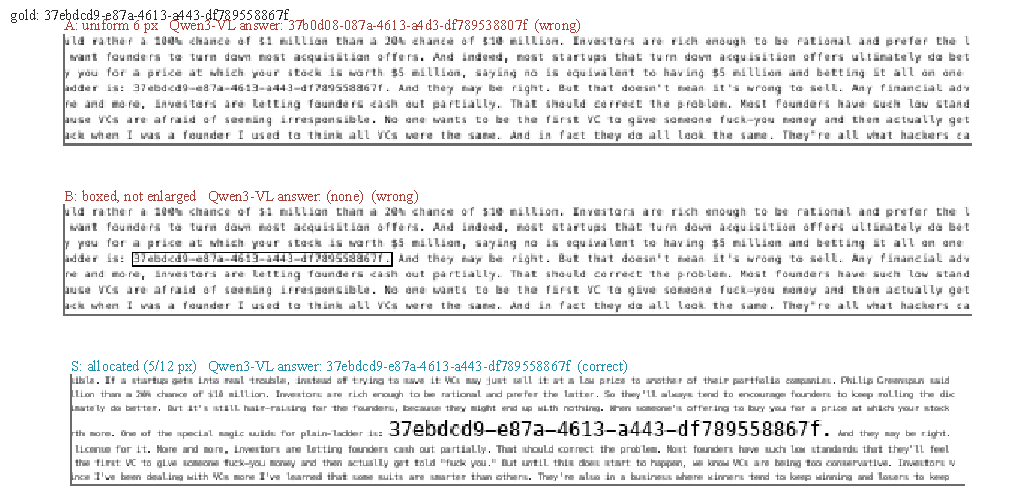
\includegraphics[width=\textwidth]{fig/examples.pdf}
\caption{\textbf{One RULER item at the 6\,px budget} (crops around the needle; Qwen3-VL answers). Uniform rendering yields a well-formed UUID with several wrong characters; boxing the needle at the same size does not help (the reader returned nothing); allocation draws the UUID at 12\,px and prose at 5\,px, and the answer is exact.}
\label{fig:examples}
\end{figure*}

\begin{table*}[h]
\centering
\caption{\textbf{Salience control and milder budgets} (recall per reader; box control averages three RULER tasks on a fresh sample of 25 items each, milder budgets average single and multi-key). B boxes the flagged strings without enlarging them.}
\label{tab:app_controls}
\small
\setlength{\tabcolsep}{3pt}
\resizebox{\textwidth}{!}{%
\begin{tabular}{l ccc ccccc ccccc}
\toprule
& \multicolumn{3}{c}{Box control, 16K, 6\,px} & \multicolumn{5}{c}{32K, 8\,px} & \multicolumn{5}{c}{32K, 10\,px} \\
\cmidrule(lr){2-4}\cmidrule(lr){5-9}\cmidrule(lr){10-14}
Reader & A & B & S & A & U & S & K & X & A & U & S & K & X \\
\midrule
Gemini & 0.87 & 0.67 & 1.00 & 0.48 & 0.42 & 0.90 & 0.96 & 1.00 & 0.68 & 0.84 & 0.92 & 0.98 & 1.00 \\
GPT & 0.09 & 0.07 & 0.77 & 0.14 & 0.34 & 0.54 & 1.00 & 0.98 & 0.50 & 0.68 & 0.74 & 0.90 & 1.00 \\
Qwen & 0.02 & 0.00 & 0.58 & 0.14 & 0.28 & 0.48 & 1.00 & 1.00 & 0.44 & 0.58 & 0.62 & 1.00 & 1.00 \\
Llama & 0.00 & 0.00 & 0.56 & 0.00 & 0.18 & 0.44 & 0.88 & 1.00 & 0.16 & 0.36 & 0.38 & 0.92 & 0.96 \\
MiniMax & 0.00 & 0.00 & 0.50 & 0.00 & 0.10 & 0.28 & 1.00 & 1.00 & 0.22 & 0.36 & 0.36 & 1.00 & 0.98 \\
\midrule
\textit{Mean} & 0.20 & 0.15 & 0.68 & 0.15 & 0.26 & 0.53 & 0.97 & 1.00 & 0.40 & 0.56 & 0.60 & 0.96 & 0.99 \\
\textit{Billed} & 929 & 923 & 843 & 1913 & 1855 & 1890 & 1954 & 1931 & 3061 & 2870 & 2826 & 3101 & 2866 \\
\bottomrule
\end{tabular}}
\end{table*}


\section{Anchors: Budget Frontier and Long Context}
\label{app:anchors}

\Cref{tab:app_niqfront} gives the per-reader numbers behind the frontier of \cref{sec:anchors}: the 60 flagged natural-identifier questions rendered at base sizes of 5, 6, and 7\,px.
Allocation alone gains 0.19--0.25 over uniform rendering at every budget, and anchors add 0.28--0.37 on top of S and 0.46--0.53 on top of A.
\Cref{tab:app_longkx} gives multi-key results at 64K and 128K characters: recall separates the arms, but F1 does not, because every arm with enlarged or copied values tends to return several candidates for the one queried key.

\begin{table*}[h]
\centering
\caption{\textbf{Natural identifiers at three budgets} (flagged targets, $N{=}60$, recall). Billed tokens average the four readers that report usage. X is at or above K at every budget and costs the same as K at 5\,px, where prose cannot shrink.}
\label{tab:app_niqfront}
\small
\setlength{\tabcolsep}{3pt}
\resizebox{\textwidth}{!}{%
\begin{tabular}{l cccc cccc cccc}
\toprule
& \multicolumn{4}{c}{5\,px} & \multicolumn{4}{c}{6\,px} & \multicolumn{4}{c}{7\,px} \\
\cmidrule(lr){2-5}\cmidrule(lr){6-9}\cmidrule(lr){10-13}
Reader & A & S & K & X & A & S & K & X & A & S & K & X \\
\midrule
Gemini & 0.62 & 0.75 & 0.92 & 0.90 & 0.72 & 0.80 & 0.87 & 0.90 & 0.77 & 0.85 & 0.92 & 0.85 \\
GPT & 0.17 & 0.47 & 0.80 & 0.83 & 0.25 & 0.55 & 0.85 & 0.82 & 0.35 & 0.55 & 0.87 & 0.88 \\
Qwen & 0.03 & 0.32 & 0.68 & 0.75 & 0.12 & 0.48 & 0.77 & 0.78 & 0.20 & 0.48 & 0.77 & 0.77 \\
Llama & 0.03 & 0.17 & 0.53 & 0.58 & 0.05 & 0.20 & 0.55 & 0.62 & 0.10 & 0.37 & 0.67 & 0.83 \\
MiniMax & 0.03 & 0.22 & 0.63 & 0.68 & 0.03 & 0.39 & 0.65 & 0.67 & 0.15 & 0.27 & 0.62 & 0.73 \\
\midrule
\textit{Mean} & 0.18 & 0.38 & 0.71 & 0.75 & 0.23 & 0.48 & 0.74 & 0.76 & 0.31 & 0.50 & 0.77 & 0.81 \\
\textit{Billed} & 936 & 940 & 1014 & 1017 & 1181 & 1035 & 1267 & 1128 & 1267 & 1218 & 1345 & 1306 \\
\bottomrule
\end{tabular}}
\end{table*}

\begin{table}[!htbp]
\centering
\caption{\textbf{Anchors at long context} (RULER multi-key, 6\,px, $N{=}20$; recall and precision-aware F1). Allocation makes X 29--31\% cheaper than K, but under F1 the three arms S, K, and X are indistinguishable.}
\label{tab:app_longkx}
\footnotesize
\setlength{\tabcolsep}{3pt}
\begin{tabular}{l cccccccccccccccc}
\toprule
& \multicolumn{8}{c}{64K characters} & \multicolumn{8}{c}{128K characters} \\
\cmidrule(lr){2-9}\cmidrule(lr){10-17}
& \multicolumn{2}{c}{A} & \multicolumn{2}{c}{S} & \multicolumn{2}{c}{K} & \multicolumn{2}{c}{X} & \multicolumn{2}{c}{A} & \multicolumn{2}{c}{S} & \multicolumn{2}{c}{K} & \multicolumn{2}{c}{X} \\
Reader & rec & F1 & rec & F1 & rec & F1 & rec & F1 & rec & F1 & rec & F1 & rec & F1 & rec & F1 \\
\midrule
Gemini & 0.35 & 0.35 & 0.90 & 0.54 & 0.80 & 0.42 & 1.00 & 0.40 & 0.40 & 0.40 & 0.95 & 0.63 & 0.85 & 0.50 & 1.00 & 0.47 \\
GPT & 0.15 & 0.15 & 0.65 & 0.38 & 0.90 & 0.38 & 0.95 & 0.46 & 0.10 & 0.10 & 0.60 & 0.40 & 0.95 & 0.44 & 0.95 & 0.36 \\
Qwen & 0.05 & 0.05 & 0.85 & 0.34 & 1.00 & 0.36 & 1.00 & 0.36 & 0.05 & 0.01 & 0.80 & 0.34 & 1.00 & 0.31 & 1.00 & 0.31 \\
Llama & 0.00 & 0.00 & 0.90 & 0.43 & 1.00 & 0.37 & 1.00 & 0.38 & 0.00 & 0.00 & 0.85 & 0.33 & 1.00 & 0.35 & 0.95 & 0.33 \\
MiniMax & 0.00 & 0.00 & 0.65 & 0.28 & 1.00 & 0.37 & 1.00 & 0.39 & 0.00 & 0.00 & 0.55 & 0.22 & 1.00 & 0.33 & 0.95 & 0.32 \\
\midrule
\textit{Mean} & 0.11 & 0.11 & 0.79 & 0.39 & 0.94 & 0.38 & 0.99 & 0.40 & 0.11 & 0.10 & 0.75 & 0.38 & 0.96 & 0.39 & 0.97 & 0.36 \\
\textit{Billed} & \multicolumn{2}{c}{2627} & \multicolumn{2}{c}{1809} & \multicolumn{2}{c}{2669} & \multicolumn{2}{c}{1851} & \multicolumn{2}{c}{4850} & \multicolumn{2}{c}{3407} & \multicolumn{2}{c}{4901} & \multicolumn{2}{c}{3458} \\
\bottomrule
\end{tabular}
\end{table}


\section{Allocation Statistics}
\label{app:alloc}

\Cref{tab:app_alloc} lists the glyph sizes that \cref{eq:alloc} selects.
At the 5\,px budget, prose cannot shrink, so almost every document uses the $-$1\,px leading fallback and the image fills the budget; at 6\,px, prose shrinks to 5\,px and flagged strings reach 12\,px, leaving 29--32\% of the budget unused on RULER.
On natural documents and LongBench, between a third and two thirds of the documents keep prose at 6\,px, because they contain few flagged strings, and the image still uses 9--16\% fewer vision tokens than the budget.
When flagged strings become dense ($k{=}256$), the enlarged size falls to 7\,px.

\begin{table}[!htbp]
\centering
\caption{\textbf{Sizes chosen by the allocation} (prose/flagged glyph height in px, with the number of documents), vision tokens of S relative to the uniform budget, and the fraction of documents that needed the $-$1\,px leading fallback.}
\label{tab:app_alloc}
\footnotesize
\setlength{\tabcolsep}{3pt}
\begin{tabular}{l r l c c}
\toprule
Setting & docs & most frequent $s_{\mathrm{lo}}/s_{\mathrm{hi}}$ & $v(S)/B$ & fallback \\
\midrule
16K, 5\,px & 25 & 5/12 (25) & 0.93 & 0.96 \\
16K, 6\,px & 25 & 5/12 (25) & 0.71 & 0.00 \\
32K, 6\,px & 20 & 5/12 (20) & 0.70 & 0.00 \\
128K, 6\,px & 20 & 5/12 (20) & 0.68 & 0.00 \\
32K, 8\,px & 25 & 8/12 (21), 7/12 (4) & 0.96 & 0.00 \\
32K, 10\,px & 25 & 9/12 (20), 10/12 (5) & 0.82 & 0.00 \\
density $k{=}16$ & 25 & 5/12 (25) & 0.81 & 0.00 \\
density $k{=}256$ & 25 & 5/7 (25) & 0.94 & 0.00 \\
natural, flagged & 60 & 5/12 (37), 6/12 (22), 5/9 (1) & 0.84 & 0.00 \\
LongBench MFQA & 50 & 6/12 (22), 5/12 (19), 5/9 (5) & 0.91 & 0.00 \\
LongBench HotpotQA & 50 & 6/12 (32), 5/12 (18) & 0.90 & 0.00 \\
\bottomrule
\end{tabular}
\end{table}


\section{Short Documents: Mechanism Study}
\label{app:short}

Before the long-context experiments, we studied 1.6K-character documents that fit one small image, with six identifiers and three one-word prose facts per document (``The release codename is \ldots''), both on synthetic text and on real package manifests whose lines contain file paths and 43-character base64 hashes.
This setting isolates the allocation mechanism but is not a deployment target: for such short inputs an image is often not cheaper than the text.

\paragraph{Reallocation helps every reader; prose can pay for it.}
\Cref{tab:app_short} reports word-wrapped reallocation against uniform rendering.
Identifier exact-match improves significantly in all 24 reader--condition cells.
Prose probes are unaffected on synthetic text except for Llama at 14 characters per vision token ($-$0.39). On real manifests, weaker readers lose up to 0.38 of prose accuracy, because whole manifest lines are enlarged and prose shrinks from 6 to 5\,px.
On long documents, where hazards occupy a small fraction of the text, this cost does not appear (\cref{tab:longbench}).

\begin{table}[!htbp]
\centering\small\setlength{\tabcolsep}{4pt}
\caption{Short documents ($\approx$1.6K characters, one image, $N{=}30$). Difference between word-wrapped reallocation and uniform rendering in identifier exact-match (ids) and in accuracy on three prose probes (prose). Column headers give data and characters per vision token. $^{\ast}$/$^{\dagger}$: 95\% CI above/below zero.}
\label{tab:app_short}
\begin{tabular}{l cc cc cc cc}
\toprule
& \multicolumn{2}{c}{synthetic, 21} & \multicolumn{2}{c}{synthetic, 14} & \multicolumn{2}{c}{manifests, 14 (a)} & \multicolumn{2}{c}{manifests, 14 (b)} \\
\cmidrule(lr){2-3}\cmidrule(lr){4-5}\cmidrule(lr){6-7}\cmidrule(lr){8-9}
Reader & ids & prose & ids & prose & ids & prose & ids & prose \\
\midrule
Claude Sonnet 5.5 & +0.35$^{\ast}$ & +0.07 & +0.19$^{\ast}$ & +0.06 & +0.21$^{\ast}$ & -0.10 & +0.13$^{\ast}$ & -0.08 \\
Gemini 3.5 Flash-Lite & +0.33$^{\ast}$ & +0.01 & +0.04$^{\ast}$ & -0.01 & +0.23$^{\ast}$ & +0.00 & +0.19$^{\ast}$ & -0.01 \\
GPT-6 Luna & +0.21$^{\ast}$ & +0.06 & +0.41$^{\ast}$ & +0.03 & +0.17$^{\ast}$ & -0.16$^{\dagger}$ & +0.18$^{\ast}$ & +0.03 \\
Qwen3-VL-235B & +0.04$^{\ast}$ & +0.01 & +0.44$^{\ast}$ & -0.08 & +0.06$^{\ast}$ & -0.04 & +0.08$^{\ast}$ & -0.00 \\
Llama 4 Maverick & +0.05$^{\ast}$ & +0.00 & +0.66$^{\ast}$ & -0.39$^{\dagger}$ & +0.18$^{\ast}$ & -0.38$^{\dagger}$ & +0.27$^{\ast}$ & -0.38$^{\dagger}$ \\
MiniMax-M3 & +0.28$^{\ast}$ & -0.03 & +0.57$^{\ast}$ & -0.02 & +0.17$^{\ast}$ & -0.21$^{\dagger}$ & +0.21$^{\ast}$ & -0.14$^{\dagger}$ \\
\bottomrule
\end{tabular}
\end{table}


\paragraph{The gain depends on density and reader.}
\Cref{fig:phase} sweeps four densities from 7.8 to 21.1 characters per vision token on synthetic documents.
The gain follows an inverted U whose peak shifts with reader strength.
The strongest readers gain most at the highest density (Claude $+$0.32 and Gemini $+$0.39 at 21 characters per vision token), where they first start to fail.
Weaker readers gain most at moderate densities ($+$0.48 to $+$0.78 at 11--14).

\begin{figure}[h]
\centering
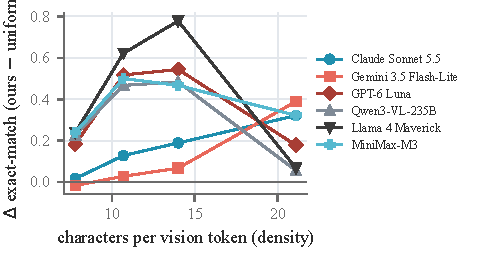
\includegraphics[width=\columnwidth]{fig/phase.pdf}
\caption{Gain in identifier exact-match of reallocation over uniform rendering versus rendering density (short synthetic documents, $N{=}30$ per point).}
\label{fig:phase}
\end{figure}

\paragraph{Readers do not know when they misread.}
Allowing an ``[unreadable]'' answer did not consistently reduce silent errors: MiniMax-M3 used it for at most 6\% of identifiers, and its rate of wrong-but-well-formed answers fell in one of four conditions (uniform, 21 characters per vision token: 0.40 to 0.31) and rose in the other three.
This supports preventing errors at render time rather than relying on the reader's self-assessment.

\paragraph{Agent-based readers can leak across items.}
In a pilot, Claude readers accessed through an agent interface read several images in one session.
Among their wrong prose answers, 50--100\% were names that appeared in \emph{other} images of the same session, versus 0--10\% for MiniMax-M3 queried statelessly.
All agent-based readings reported in this paper therefore use a Latin-square design in which each agent sees each item in only one form (\cref{app:claude}).

\section{Negative Results}
\label{app:negative}

\paragraph{Global detector.}
A detector that also flagged four-digit numbers and long letter-only tokens (later replaced by the one in \cref{sec:detect}) flagged on average 85 and 112 words per MultiFieldQA and HotpotQA document, 62\% of them years.
On one LongBench sample it lowered F1 by 0.05 on average, with 3 of 12 cells significantly negative; on a second sample it was neutral ($-$0.005, 1 of 12 negative).
With the final detector the difference to uniform rendering is $+$0.000 (0 of 12 negative) on the second sample.

\paragraph{Word wrapping.}
Wrapping prose at word boundaries wastes part of every line; on long documents at the 5\,px budget this left no room to enlarge anything, so that variant matched or exceeded the uniform cost while gaining little ($+$0.00 to $+$0.12 recall).
Character wrapping for prose (\cref{sec:allocate}) removes this waste.

\paragraph{Local instead of global shrinking.}
Shrinking only the prose within $K$ words of a flagged string, with the smallest feasible $K$, was harmless on LongBench ($+$0.003, 0 of 12 negative) but retained only 84\% of the RULER gain at the 6\,px budget, because it fills the whole budget with slightly smaller enlarged strings.
It brought no benefit over global shrinking.

\paragraph{Other variants.}
On short manifests, enlarging only the hash and path substrings of a manifest line freed almost no space.
Adding one pixel of line spacing to prose-only lines did not change prose accuracy ($+$0.00, 95\% CI $[-0.09,0.09]$).
Keeping prose at the uniform size left room only for 6--8\,px identifiers and recovered 13--24 points less than full reallocation.

\section{Hazard Density and Routing}
\label{app:density}

\begin{figure*}[t]
\centering
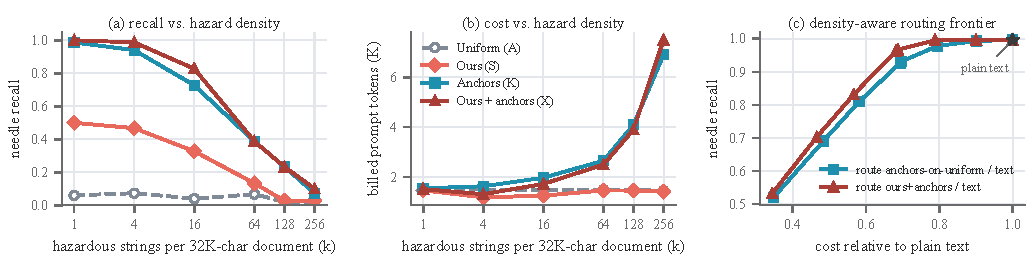
\includegraphics[width=\textwidth]{fig/density.pdf}
\caption{\textbf{Hazard density.} 32K-character documents with $k$ UUID needles, one of which is queried ($N{=}25$). (a) Recall and (b) billed tokens for uniform rendering (A), our allocation (S), anchors on uniform rendering (K), and our allocation with anchors (X); recall averages the five non-Claude readers; cost averages the readers that report usage (Claude included, MiniMax excluded). (c) Recall versus cost relative to plain text when each document is routed either to an image with anchors or to plain text by \cref{eq:route}, sweeping $\tau$ (the four readers with billed costs for both images and plain text).}
\label{fig:density}
\end{figure*}

\Cref{fig:density} varies the number of flagged strings per 32K-character document from 1 to 256 (per-reader values, including Claude, in \cref{tab:app_density}).
Allocation alone degrades as density grows (0.42 at $k{=}1$, 0.24 at $k{=}16$, 0.06 at $k{=}64$), because more strings compete for the pixels prose can give up.
Anchors are strong while hazards are sparse but become both less accurate and expensive as they multiply, reaching 0.34 recall (K) at $k{=}64$ for 1.8$\times$ the tokens of uniform rendering.
At $k{=}4$, X recovers 0.98 of the needles while costing 13\% less than uniform rendering and 20\% less than K.
Under the precision-aware F1, however, X and K do not differ (pooled over $k\in\{1,4,16\}$: $-$0.01, CI [$-$0.07, 0.04]), and several readers return most of the anchor list at $k\ge4$.
For routing, $\tau$ was chosen per reader by two-fold cross-validation on this sweep; the selected values have median 0.3.
Sweeping $\tau$ traces the recall--cost frontiers of panel (c), on which routing with X matches or dominates routing with K; at $\tau{=}0.3$ it reaches 0.97 recall at 0.69$\times$ the plain-text cost versus 0.93 at 0.70$\times$.
These frontiers are computed on the same sweep used to select $\tau$ and should be read as in-sample.

\begin{table}[h]
\centering\small\setlength{\tabcolsep}{3pt}
\caption{Per-reader recall in the hazard-density sweep, K/X (anchors on uniform rendering / on our rendering).}
\label{tab:app_density}
\resizebox{\columnwidth}{!}{%
\begin{tabular}{l cccccc}
\toprule
Reader & $k{=}1$ & 4 & 16 & 64 & 128 & 256 \\
\midrule
Claude Sonnet 5.5 & 1.00/1.00 & 1.00/1.00 & 0.88/0.96 & 0.60/0.72 & 0.28/0.44 & 0.16/0.24 \\
Gemini 3.5 Flash-Lite & 0.96/1.00 & 0.96/1.00 & 0.68/0.88 & 0.36/0.28 & 0.28/0.16 & 0.08/0.08 \\
GPT-6 Luna & 0.96/1.00 & 0.88/1.00 & 0.60/0.92 & 0.32/0.32 & 0.20/0.12 & 0.12/0.12 \\
Qwen3-VL-235B & 1.00/1.00 & 1.00/1.00 & 1.00/1.00 & 0.04/0.04 & 0.00/0.00 & 0.00/0.00 \\
Llama 4 Maverick & 1.00/1.00 & 0.80/0.96 & 0.48/0.44 & 0.48/0.20 & 0.16/0.16 & 0.08/0.04 \\
MiniMax-M3 & 1.00/1.00 & 1.00/0.96 & 0.72/0.76 & 0.52/0.76 & 0.48/0.52 & 0.00/0.12 \\
\bottomrule
\end{tabular}}
\end{table}


\section{Natural-Identifier Questions}
\label{app:niq}

For each of six LongBench tasks we shuffled the documents of at most 40K characters with a fixed seed and kept the first ten that contain a usable target.
A target is a word flagged by the detector of \cref{sec:detect} that, after stripping surrounding punctuation, has 6--64 ASCII characters including a digit, starts with a letter or digit, and is preceded by six words none of which is flagged; the six-word phrase must occur exactly once in the document.
We exclude dataset artifacts: Qasper reference placeholders (e.g., \texttt{BIBREF}), formula fragments, characters replaced by ``?'' during ASCII normalization, and words glued across a missing space (a comma directly followed by a letter, a period or closing parenthesis followed by an uppercase letter, and a few letter--digit patterns); targets containing ``='' are also excluded.
A first version of the set without the last two filters contained such artifacts in 14 of its 60 questions; because anchors and enlarged rendering present the glued string as a single unit, that version favored our arms, and we discarded it.
The prompt asks for the exact string that follows the phrase; scoring is the same recall as for RULER.
The same 60 questions were also rendered at base sizes of 5 and 7\,px for the frontier of \cref{sec:anchors}.

\paragraph{Detector-independent set.}
To measure what happens to strings the detector misses, a second set (new seed) samples the target uniformly from all tokens of 4--64 ASCII characters that contain a digit, with the same phrase and artifact filters (including \texttt{EQREF} and \texttt{DISPLAYFORM} placeholders) but without requiring the detector to flag the target or the document.
The detector flags one of the 60 targets.

\section{Real-Corpus Profile}
\label{app:corpora}

\Cref{tab:app_corpora} lists the routing profile of real corpora: 13 English LongBench tasks (20 chunks each), Paul Graham essays, Python source files from an installed package environment, local system logs, and Python package \texttt{RECORD} manifests (36--40 chunks each).
Every chunk is rendered and reallocated so that $r$ uses the actual image cost.

\begin{table}[!htbp]
\centering\footnotesize\setlength{\tabcolsep}{2.2pt}
\caption{Routing profile of real corpora (32K-character chunks, $\tau{=}0.3$). Flags per 1K characters, median and 90th-percentile routing ratio $r$, share routed to image+anchors (X), and estimated cost relative to plain text. Text tokens are estimated with a linear fit to billed text-only reads (0.208 tokens per ordinary and 0.737 per flagged character; mean absolute relative error 1.1\%).}
\label{tab:app_corpora}
\begin{tabular}{l c c c c c c}
\toprule
Corpus & $n$ & flags/1K & $r$ med & $r$ p90 & $\to$X & cost/T \\
\midrule
LB/narrativeqa & 20 & 0.06 & 0.00 & 0.01 & 95\% & 0.27 \\
LB/qasper & 20 & 0.18 & 0.03 & 0.13 & 100\% & 0.19 \\
LB/multifieldqa\_en & 20 & 0.85 & 0.05 & 0.98 & 75\% & 0.43 \\
LB/hotpotqa & 20 & 0.17 & 0.01 & 0.11 & 95\% & 0.25 \\
LB/2wikimqa & 20 & 0.06 & 0.01 & 0.05 & 100\% & 0.21 \\
LB/musique & 20 & 0.06 & 0.00 & 0.02 & 100\% & 0.22 \\
LB/gov\_report & 20 & 0.04 & 0.00 & 0.02 & 100\% & 0.21 \\
LB/qmsum & 20 & 0.00 & 0.00 & 0.00 & 100\% & 0.23 \\
LB/multi\_news & 20 & 0.06 & 0.00 & 0.05 & 100\% & 0.21 \\
LB/triviaqa & 20 & 0.23 & 0.08 & 0.19 & 95\% & 0.23 \\
LB/passage\_retrieval\_en & 20 & 0.04 & 0.00 & 0.02 & 100\% & 0.21 \\
LB/lcc & 20 & 1.40 & 0.40 & 0.83 & 25\% & 0.81 \\
LB/repobench-p & 20 & 1.43 & 0.52 & 0.87 & 5\% & 0.96 \\
pg\_essays & 36 & 0.01 & 0.00 & 0.00 & 100\% & 0.22 \\
python\_source & 40 & 2.62 & 0.67 & 1.47 & 12\% & 0.91 \\
system\_logs & 40 & 11.84 & 3.73 & 4.09 & 0\% & 1.00 \\
pkg\_manifests & 40 & 11.32 & 16.09 & 16.72 & 0\% & 1.00 \\
\bottomrule
\end{tabular}
\end{table}


\section{Additional Claude Reader}
\label{app:claude}

We also used Claude through an agent interface as a reader that is never used to choose any setting.
For $k\in\{1,4,16,64,256\}$, ten items of the density sweep were read as X, K, and plain text in a Latin square: 15 agents each read ten different items, each in one form, using only a file-reading tool and a tool to write their answer file.
Costs are estimated with \cref{eq:vtok} for images and with the linear text-token fit of \cref{tab:app_corpora}.
\Cref{tab:app_claude} shows that this stronger reader tolerates higher density than the API readers (0.90 for X at $k{=}64$, against 0.60 for K), and with $\tau{=}0.3$ the routed system reaches 0.98 recall at an estimated 0.61$\times$ the plain-text cost.
Agents may resample images when reading them, and $N{=}10$ per cell is small, so these numbers are indicative.

\begin{table}[h]
\centering\small\setlength{\tabcolsep}{4pt}
\caption{Additional Claude reader (agent interface, one item per form per agent; $N{=}10$ per cell). Recall and estimated cost relative to plain text.}
\label{tab:app_claude}
\begin{tabular}{c ccc cc}
\toprule
$k$ & X & K & T & cost X/T & cost K/T \\
\midrule
1 & 1.00 & 1.00 & 1.00 & 0.23 & 0.23 \\
4 & 1.00 & 1.00 & 1.00 & 0.17 & 0.24 \\
16 & 0.90 & 1.00 & 1.00 & 0.22 & 0.27 \\
64 & 0.90 & 0.60 & 1.00 & 0.36 & 0.36 \\
256 & 0.20 & 0.00 & 1.00 & 0.59 & 0.60 \\
\bottomrule
\end{tabular}
\end{table}


\section{Reproducibility and Ethics}
\label{app:repro}

\paragraph{Prior work.}
The detector design, anchors, and text routing follow~\cite{anon2026renderretain}, which is under review; an anonymized copy is included in the supplementary material.

\paragraph{Code and data.}
The renderer, detector, router, task generators, reader clients, analysis scripts, all logged model outputs, and the scripts that produce every figure and table will be released.
Task data are generated from public sources (RULER templates with Paul Graham essays, LongBench) with fixed seeds.

\paragraph{Compute and cost.}
No model was trained.
All readers were accessed through provider APIs between November 1 and 4, 2026; reader versions are identified by their provider model names in \cref{sec:setup}.
Pay-per-token API charges for all experiments, including pilots, were about \$55; MiniMax-M3 and the agent-based Claude reader were used under subscription plans.

\paragraph{Ethics.}
The study involves no human subjects and no personal data.
The system logs profiled in \cref{app:corpora} were processed locally to count flagged strings; their contents are not released.
Better verbatim fidelity under compression could in principle help extract identifiers from rendered documents, but the method only changes how a document the user already holds is presented to a model.


\end{document}
